\documentclass{MScthesisITEM}

\usepackage{graphicx}
\usepackage{times}
\usepackage[utf8]{inputenc}
\usepackage{mathtools}
\usepackage{algorithm}
\usepackage{natbib}
\usepackage{datatool}
\usepackage{glossaries}
\usepackage{url}
\usepackage{hyperref}
\usepackage{longtable}

\title{Interdependent Privacy on Facebook} % The title of your assignement; NB use \newlinetitle to start a newline
\author{Esther Bloemendaal \\ Ida Malene Hassel Øveråsen}
\professor{Jan Audestad, ITEM} % Affiliation = ITEM for instance
\supervisor{Gergely Biczók, ITEM}

%% Uncomment the following in case you want subfigures; note that there will be a warning for the caption package
% \let\subcaption\undefined
% \let\subfloat\undefined
% \usepackage[bf]{caption}
% \usepackage{subcaption}

\DeclareGraphicsExtensions{.pdf,.jpg}
\graphicspath{{./figs/}}

\loadglsentries{glossary}
\makeglossaries

\begin{document}
\selectlanguage{english}
\pagenumbering{roman}
\pagestyle{plain}

%% Only for the project
\titleITEM


\selectlanguage{english}
\renewcommand{\abstractname}{Abstract}
\begin{abstract}
With the evolution of online social networks, the incentive to share personal information has grown drastically. Along with the progressive data sharing that exists in today's interconnected world, privacy concerns arise. The privacy of an individual is bound to be affected by the decisions of others, and is therefore, to some degree, out of the user's control. This phenomenon lays the basis for the term \textit{interdependent privacy}. In this study, we will direct our focus to Facebook, today's largest online social network.  

Interdependent privacy is one specific part of the privacy issues that exists on Facebook. In order to get a full overview and understanding of this matter, we have looked into different aspects of Facebook privacy. We have mapped the development of the default privacy settings and the most important features introduced by Facebook over the years. We have also looked at user awareness with regard to Facebook privacy, how much they care about their privacy, as well as their awareness regarding app permission requests.

To map human awareness, we constructed a survey. In order to get an adequate picture of people's awareness, we distributed the survey on Amazon Mechanical Turk (MTurk). This is a marketplace for work that requires human intelligence. One of the key benefits of using MTurk is that it provides one of the largest subject pools available, with both diversity and low cost. We analyzed these results with focus on awareness of privacy settings (including app settings). We wanted to see if there was a connection between privacy settings and app settings, and awareness of the permissions requested when installing apps. 

%Results: What's the answer? Give specific results.
Our results show that all our respondents at some point have changed their privacy settings, as nobody had all their settings set to default. The majority of all the respondents check their settings 3-6 times a year. When we look at the corner-points, the ones that check them frequently and those that have not checked their settings during the last year, there is a clear difference. This gave the basis for two hypotheses that we thoroughly investigate in this report. "People that check their Facebook settings seldom, do not have as private/secure settings as the ones who check their settings often. Also, these people do not have as much knowledge about app permission requests, as the ones who check their Facebook settings often" and "People with many apps have less knowledge about the app permission requests, and less knowledge about the existence of the setting "Apps others use"". 

Our research backs up both hypotheses. A higher percentage of the people checking frequently have changed their settings to a more private/secure option, meaning that they are aware of the settings' existence. These users were both younger (almost 10 years in average) and more active (almost 20\% more active), than the ones who seldom check their settings. The people checking frequently are also to a higher extent aware of the app permission requests. As well as the setting "Apps others use", which to a high extent concerns interdependent privacy. 
We also looked at the awareness of the permission requests for the ones having many apps connected to their Facebook account, versus the ones having just a few. The ones with few apps were more aware of all the requests we presented in our survey, and this group was also more aware of the existence of the setting "Apps others use", in comparison to the ones who had many apps connected to their Facebook account. 

An interesting observation was that the respondents of our survey cared more about what they post (comments, photos, etc.) about others, than what is posted about themselves. The knowledge of the term interdependent privacy, as well as the knowledge about the app permission requests, was low.

%Conclusion: What are the implications of your answer? summary of the discussion of the results and conclusion 
The results from our research shows that our initial assumptions were correct. Specifically there exists little knowledge around the issues regarding interdependent privacy. Online privacy is a hot topic in the media these days and people do care about what is posted about them; but still they have poor security/privacy settings and in general little to no knowledge about app permissions. Is Facebook trying to hide the fact that information about you may be shared without your knowledge? If so, is this in conflict with their vision of an open and interconnected world?

\end{abstract}
\cleardoublepage


\selectlanguage{english}

\renewcommand{\abstractname}{Preface}
\begin{abstract}

This study was performed as a specialization project on behalf of the Department of Telematics at the Norwegian University of Science and Technology. The specialization project is part of two main profiles, information security and tele-economics, and this report is the final result of the project and is worth 15 ECTS points. The study was conducted between September and December 2013. The project description was outlined in cooperation with our project supervisor PhD Gergely Biczók at the Department of Telematics. 

We would like to thank Gergely Biczók who has guided us through our project, and contributed with helpful ideas, feedback and support. We would also like to thank                        everyone who answered our survey, and helped us with valuable research information. A special thanks to our friends Aurora Klæboe Berg, Kine Aasjord Omholt and Thomas Normann for sharing the survey on their Facebook page, and making the survey reach out to a wider audience.  \\
%Takke Audestad om vi får noe ut av han
\vspace*{2\baselineskip}
\paragraph{}
Trondheim, December 16, 2013
\vspace*{1.5\baselineskip}
\paragraph{}
Esther Bloemendaal
\paragraph{}
Ida Malene Hassel Øveråsen


\end{abstract}
\cleardoublepage

\tableofcontents*
\cleardoublepage

%% include if relevant
\listoffigures
\cleardoublepage

%% include if relevant
\listoftables
\cleardoublepage


%% include if relevant
\printglossary[title=List of Symbols, style=long]
\cleardoublepage
\glsaddall[]

%% include if relevant
\printglossary[title=List of Acronyms,type=\acronymtype] % prints just the list of acronyms
\cleardoublepage
\pagenumbering{arabic}

%\pagestyle{ruled}

\chapter{Introduction}
\label{chp:introduction} 

\section{Motivation}
Facebook's popularity have increased drastically since it was introduced to the public in 2006, and people share enormous amounts of information on Facebook. This makes it interesting to look into privacy issues related to Facebook, and find out how aware people are of the existence of the various settings. The introduction of applications on Facebook, introduced a whole new dimension to the privacy issues on Facebook. It is therefore also interesting to look at people's awareness when it comes to the information they share with apps, and how apps utilize this information. Previous studies has shown that the apps' permission requests often ambiguous, and that the permissions often goes against the users' privacy settings \cite{thirdPartyApps}. Facebook has for many also become a sort of "snopping"-tool and it is therefore important that the users are able to protect the information they do not want shared with the public. I order to do this they need awareness regarding the existing settings. 


\section{Problem Description}
%Har vi lov til å endre denne?
Interdependency is a reciprocal relation between two or more decision-making entities, whose actions have consequences for each other. Interdependency is a very important issue when it comes to social networks, since your privacy is affected by the privacy decision of others. This project will be directed towards the interdependent privacy issues on Facebook.
\paragraph{}
Since Facebook came out in 2006, there has been a major change in privacy and security settings. At the same time Facebook's features have been significantly upgraded (e.g., Apps), and the platform itself has expanded to several different platforms (e.g., iOS and Android). Owing to this development, the complexity of privacy-related issues has made the originally embedded privacy requirements inadequate. We are going to map and analyze this development to see how privacy settings has changed over time. We will also look at human behaviour with regard to Facebook privacy. How this affects people when it comes to, for example, personal life and future job prospects, and to what degree people are aware of the unanticipated consequences the use of Facebook can bring.
\paragraph{}
In order to carry out the behavioural research we will use Amazon Mechanical Turk, enabling us to reach a wide audience. Amazon Mechanical Turk is a marketplace for work that requires human intelligence, and works well for conducting surveys.
The key benefits of Amazon Mechanical Turk when you are conducting behavioural research is that it provides one of the largest subject pools, with both diversity and low cost. By using the results of the survey we will look into what kind of privacy settings different types of people value and map their awareness when it comes to the importance of different privacy settings. 

\section{Methodology}
\label{sec:methodology}
Our assignment is divided into parts, where one consists of collecting data from Facebook users regarding their view on Facebook privacy settings, and the other is a theoretical research of how Facebook privacy settings has evolved since the introduction of Facebook. This means that we have used different approaches to be able to retrieve the information desired.

\paragraph{Approach}
In this section we will describe our approach of collecting data from Facebook users regarding their view on Facebook privacy settings. Facebook is a global social network, so to be able to get more accurate information it is important to reach out to a wide and diverse audience. We decided to use Amazon Mechanical Turk for this purpose. To gather the data, we made a survey for the users to answer. Survey is a common used research method that involves the use of standardized questionnaires or interviews to collect data about people and their preferences, thoughts and behaviours in a systematic manner \cite{survey}. Survey, as a research method, has several advantages in comparison to other methods of doing research. Survey is a good method of retrieving unobservable data, like for example peoples attitudes, behaviours, characteristics, preferences, and demographics. Surveys are great when you want to cover a large group of people, like a country, that otherwise would be difficult to observe. With large groups and large amounts of data, surveys allows small effects to be detected, and makes it easy to compare the subgroups that may appear. Survey are in an economically sense cost effective. It is a lot cheaper for a researcher to make and send out a survey than to use other methods like experimental research. Survey as a research method also has some disadvantages. The method is often exposed to biases, like sampling bias, non-response bias, and social desirability bias. Surveys have a reputation for low responses, hence the non-response bias. This was one of the reasons for choosing AMT as a platform for publishing your survey. 

We started by implementing the survey in Amazon Mechanical Turk (AMT), but learned that the templates provided by AMT was missing some of the features we wished to include, like dividing the questions into several pages. So mainly for design purposes we chose to create our survey in SurveyMonkey. This is easily integrated with AMT and a often used option.  Using SurveyMonkey also made it a lot easier to keep track of answers and see summaries. SurveyMonkey has a great and easily understandable user interface, and made it easy to share the survey to other mediums like Facebook, to reach out to an even larger and more diverse audience. 

\paragraph{}
In AMT we set the requirements that the users had to be "Master Workers". This is users that through a good reputation has earned the title, and by setting this requirement we rule out unserious users and answers. This will save us a lot of time in the screening process. When a user chooses to take our survey, they first get some information about the purpose and incentive of the survey, and a link to SurveyMonkey to take the survey. When the survey is finished the user receives a code that they have to provide before submitting their HIT in AMT. This is an assurance for us that all users on AMT has finished the survey before they get paid. Throughout the lifetime of our survey we have changed this code, just to make sure that nobody tries to get paid without actually doing the work. When the survey is completed in a serious manner the workers get paid \$1,5. On average, the users spent 13 minutes and 37 seconds to take the survey, this gives an effective hourly rate of \$6,61.    

\section{Limitations} 
Our main limitation is the amount of time available to finalize our specialization project. We only had 4 months at our disposal. Our research analysis is based on the 250 responses we got on our survey. This is not enough to get a full and accurate image on the research area, but give a solid basis for further work. The amount of money granted for conducting the research was also limited, this mean we could not pay an unlimited amount of workers on AMT. In addition to this, it is not an infinite number of workers available on AMT. If we were to reach out to even more people, we would need to use several different arenas. Our results are only based on the analysis from the survey. We did not implement anything or create a "tool" in order to cover a wider field in our research. Even though we distributed our survey on AMT and Facebook, it is up to the user whether or not to take the survey. We had no control over the users' intentions. A normal problem with surveys is that there exists no way for us as researchers to verify that the respondents have answered in a truthful and proper manner. Another factor to have in mind, is the overlooking of valuable research data when conducting an analysis. 



\cleardoublepage


\chapter{Related Work}
\label{chp:relatedwork} 


\section{Social Network Services}
\paragraph{}
A social network service (SNS), is a platform used to establish social networks of different people. These people often share a common interest or activity \cite{SNS}. Online social networks (OSNs) is a large part of the social network services. From online social networks was first introduced until today, the popularity and complexity has grown drastically, with a hundreds of millions active users \cite{OSN}. OSNs have a peer-to-peer architecture, and therefore makes it easy for members to initiate communication with whom they want, given that they are also connected to the network. OSNs also enables the possibility for people to easily publish and retrieve information about subjects of interest \cite{DPBook}. The internet has caused the creation of several information sharing systems \cite{OSNpaper}. Among these systems are the Web and OSNs. As mentioned before, the popularity of OSNs has grown drastically, and have become among the most popular sites on the Web. With this change, there has also been a change in what is centralized and in focus. The Web is to a large extent organized around content, while OSNs on the other hand are organized around users. This change has lead to the importance of understanding user behaviour. You can say that the expansion of OSNs has lead to a shift in how context is exchanged over the Web. End users are no longer just content consumers, but now also required to be content creators and managers \cite{expectations}.

\paragraph{}
A user is often represented with a profile on OSNs. To obtain a profile the user, in most cases, must register the site. When a user is given a profile, it is normal for the user to provide information about themselves. This information could for example be date of birth, home town, sex, name (or pseudonym) and maybe a profile picture. The social network is formed when users start connecting with each other. The reason for these connections are numerous; real-life friends, real-life acquaintances, colleagues, share an interest/activity or if you are interested in the information contributed by the other user. 

\paragraph{}
Since Facebook was introduced to the public in 2006, it has grown to be the largest online social network (OSN) in the world. The growth of Facebook has made it necessary to introduce new ways to manage privacy and ensure a secure online environment. The privacy embedded in the program/app etc. is not enough to ensure such an environment, due to the interdependent privacy issues. Your privacy is to a large extent affected by the privacy decision of others. 

\section{Interdependent Privacy}
In today's society Internet is no longer a privilege, it is a human right. With the evolvement of the online social networks (OSN) the incentive to share personal information has grown drastically. People create profiles at different OSNs and share personal information, pictures and comments with each other. With the enormous data sharing privacy concerns arise. The privacy of an individual users i bound to be affected by the decisions of others. and therefore out of the individuals control. This phenonomen lays the basis for the term \textit{interdependent privacy} \cite{InterdependetPriv}. 

\paragraph{Privacy}
Roger Clarke defines privacy as \textit{the interest that individuals have in sustaining a 'personal space', free from interference by other people and organisations} \cite{privacy}. Further Clarke divides privacy into multiple levels; bodily, personal behaviour, information privacy. Bodily privacy is concerned with the integrity of an individual's body, such as blood transfusion without consent, compulsory immunisation and compulsory sterilisation. Personal behaviour privacy relates to all aspects of behaviour, like sexual preferences, and political and religious actions. Information privacy is a collective term including personal communication and privacy of personal data. These include the ability to communicate, using the desired media without being monitored by others, and claim that data about themselves not automatically should be available to others, even when there is data that should be processed by others.

In this article our focus will be on online privacy, the level of privacy and security of personal data published on the internet. For a user the privacy and anonymity is the most important factor in consideration when using online services. It is a hot topic and now more important than ever, especially when the consequences are unforeseen, and the extent of them are often hard to predict. Biczók and China defines online privacy risks with the basis in Clark's privacy definition as described in the list below \cite{InterdependetPriv};

\begin{itemize} 
\item Personal: Potential loss of information about a user and his/hers behavioural data. This can be done by phishing, hacking to steal secure and sensitive user data, like passwords and pin codes.
\item Relational: Revelation of how a user relate to and communicate with others. Spyware is an offline application that can obtain a users data without the consent of the user. 
\item Spatial: Invasion of  the virtual space of an online user. An example of this can be unwanted comments and posts on a user's blog or social networking page.
\end{itemize}

\paragraph{Social networking privacy}
epic.org/privacy/socialnet

\paragraph{Interdependent privacy}
In today's interconnected world, we share enormous amounts of data every single day. Protecting personal, relational and spatial privacy of individuals is no longer just dependant of only your individual actions, but increasingly depending on the actions of others \cite{InterdependetPriv}. With the continuous growing use of social networks, data sharing has become very easy. We share photos, comments, videos, and links. This increasing data sharing arises the concerns for interdependent privacy. 
 
An example can be if Alice posts and tags a picture of her Facebook friend Bob. Alice finds the picture of Bob funny and sees no problem in posting it. Bob on the other hand, does not share Alice's opinion, he finds the picture embarrassing and inappropriate. Bob wants the picture removed, but by the time Alice comes around to remove it, people have already seen it, and maybe reposted it. Bob's privacy was dependent on what Alice did, and out of his own control. 
 
Sharing information without consent from the users can lead to the emergence of externalities. In economics externalities is defined as the unintended costs or benefits that are imposed on unsuspecting people and that results from economic activity initiated by others \cite{externalityDef}. When the effect is beneficial it is considered a positive externality. A negative externality is when the side-effect is negative. Let us relate this to our example with Alice and Bob. When Alice shares the photo without Bob's consent, it might be at benefit for Alice (in personolized experience), but for Bob it will be received as a negative externality, a loss of his online privacy.  
Another example of interdependent privacy is the Facebook platform for third-party applications (apps). How your privacy depend not only on your actions, but also on the actions of your friends. We will discuss this in more detail below.   

\paragraph{}
(Her skal vi skrive kort om Facebook sin app-platform)

\paragraph{}
The article "Third-Party Apps on Facebook: Privacy and the Illusion of Control" was written in the end of 2011 and looks at the privacy threats with the use of third-party apps on Facebook \cite{thirdPartyApps}. In this paper the authors look at what information the third-party applications request when you install them, and how easy it is for an application to retrieve more information from a user than what the user initially want to. There has not been done any other studies on this topic before the time this article was written. Their aim is to increase user control of the apps' data control and alert the users when the apps' violate your initial privacy setting. When a user wants to add an application, the application is required to ask for permission to access certain information, like your "basic information", which includes name, profile picture, gender, networks, list of friends and other information that a user has publicly available to everyone. Other permissions that apps frequently ask for is "post to my wall", "send me email" and "access my profile information". You can later go to your settings and change what information you share with the apps. But by this time you may already have shared information that you initially wanted to keep private. As an example say that a user, we call her Alice, would like to keep her birthday private and have stated this in her privacy settings. Alice then install an app called "Happy Calendar", that let her keep track of friends' birthdays. When installing the app, they asked for permission to access hers and her friends' birthdays in addition to her basic information. Alice allows the app premission, to later find out that "Happy Calendar" has created an album with a calendar image showing the profile pictures to all her friends including herself. This album was posted on her wall and Alice's friends receives notifications about the album. The birthday that Alice initially wanted to keep private is no longer private. The article states that there should be more evident to the user when the app ask for information that is in conflict with the user's privacy settings. In the article two new designs of the approval page are presented and tested.  From the tests it was clear that users was not always aware of what they share, and that a more extensive and informative permission-page would be necessary. It is important that the users understand what they are sharing and that apps often ask for information that you do not want others to see.


\section{The History of Facebook}
When Mark Zuckerberg enrolled at Harvard in 2002, he had decided to major in psychology. “I just think people are the most interesting thing—other people,” he said. “What it comes down to, for me, is that people want to do what will make them happy, but in order to understand that, they really have to understand their world and what is going on around them” \cite{MeMedia}. He showed an interest and passion to connect people together and create Harvard more open. 

\begin{figure}[h!]
\centering

\includegraphics[width=0.2\textwidth]{facebook-icon.png}
\caption{The Facebook Icon}
\end{figure}

\paragraph{}
It all started in October 2003 when the Harvard sophomore Mark Zuckerberg and three of his classmates created the web page Facemash. Zuckerberg hacked into the administrative database to extract the ID photos of all the students of the different houses. The web page presented two and two photos creating a “hot or not” game for his fellow students. The votes were counted and created a top-ten list of the cutest people in each house. Within the first hour Facemash had 450 visitors and 22 000 votes. After numerous complaints from professors and fellow students, Harvard administration shut down Zuckerberg's Internet connection after a few days. Harvard charged Zuckerberg for violating individual privacy, violating privacy and breach of security for stealing the photos. Zuckerberg agreed to take the web page down and got away with just a warning.

\paragraph{}
After Facemash, Zuckerburg was known around campus as a programming prodigy. Harvard seniors, Tyler and Cameron Winklevoss and Divya Narendra had since 2002 been working on a social networking page, called HarvardConnection. This was a page where students could create a profile, and through that share some personal information and post pictures and share this with large and small communities that one could be part off. They wanted Zuckerberg's help to finalize their project so that the page could be up and running before they graduated. Zuckerberg agreed to help at the same time as pursuing his own projects. Harvard offers a class directory to all freshmen, this directory is also known as the "Facebook". This "Facebook" contains a picture of all the students, name, date of birth, home town and high school. The purpose of the "Facebook" was that the freshmen could get to know each other. Harvard's plan was to eventually get this online. Since Harvard had not gotten to it yet,  Zuckerburg decided to do the job himself. He wanted to create a page where people signed up and created their own profiles, and in that way could post some personal information about themselves, and have control over what was posted. After ten days of intensive work, Zuckerberg almost finished the site. The site was kept simple and intuitive, and everybody with a Harvard e-mail address could create a profile. The profile consisted of a profile picture, name and some personal information such as taste in books, music, films and favourite quotes. Users could link to their friend's profiles and by using a "poke" button let others know that you have visited their profile. Thefacebook went public February 4, 2004, and to get the word spread they sent it out on the Kirkland house mailing list, that contained over 300 students. It did not take long until the other houses heard and within twenty-four hours, close to fifteen hundred people ha registered. “I think it’s kind of silly that it would take the university a couple of years to get around to it,” he said. “I can do it better than they can, and I can do it in a week.” \cite{MeMedia}. Later the same year the three founders of HarvardConnection, now called ConnectU, filed a lawsuit against Zuckerburg. Stating that he broke their oral contract, stole their idea, and delayed working on their site to be able to finish his own site, Thefacebook, first. Zuckerburg denied doing anything wrong, and stated that he had proof that he did not steal the idea from the HarvardConnection. Just a few months later Facebook filed a countersuit. Facebook accused ConnectU with defamation. The case went on for years. In 2011 the Winklevoss brothers dropped the lawsuit and accepted a $ 65 $ million settlement \cite{droppLawsuit}.

\paragraph{}
There was already similar pages out there, like Friendster and myspace.com. Especially on myspace.com people played roles, giving themselves out to be someone else. Teenage girls pretending to be older and grown men giving themselves out to be young girls. There is nowhere to validate that the person really is who they give themselves out to be. This limits to what extent people posts personal information. With Thefacebook.com you had to sign up with a valid Harvard e-mail address, in that way you know that they are actual people, and mostly students. This made it easier to post more personal information like cell-phone number, home address and even sexual orientation. The concern was not about security, but more about wasting time, it became an addictive pleasure. 

\paragraph{}
It didn't take long before Mark Zuckerberg began to receive e-mails from other colleges, requesting to get Thefacebook at their schools. The site was easily scalable, the concern rather laid in how to maintain the intimacy and the clubby appeal. When Thefacebook expanded to the colleges Colombia, Yale and Stanford, students were only able to search and see people from their respective college. Only with permission from a student from another college could you add the person to your friend list. This is a key factor to Facebook's success. Zuckerberg wanted people to post personal information and create a more open school community.

\paragraph{}
In June 2004, when the school year was over, Thefacebook had expanded to over forty schools, with 150 000 users. With the rapid expansion, the need for investors and more capacity increased. Zuckerburg moved his base to California and removed the "the" from the name. Thefacebook became just Facebook.

October 2005 Facebook expanded to universities in England, Mexico and Puerto Rico, and in September 2005 a high school version was available \cite{FacebookHistory}. This was a big step for Facebook. All high school members needed an invitation to be able to join. Zuckerburg launched the possibility for all users to see the profiles and send friend request to everyone in the network, the older users had strong objections. College students did not like the idea of high school kids looking at their profiles and being able to befriend them. But with the rapid expansion Facebook was forced to make the site more open and knock down some of the walls dividing the users. Facebook made it possible for employees at different companies like Apple and Microsoft to join the network. 
At the end of 2005 Facebook was used at over 2000 colleges and at over 25 000 high schools in United states, Canada, Mexico, England, Australia, New Zealand and Ireland. 

Up to this point you had to be a student at a college of high school, or employee at a certain company to be able to join the network. After September 2006 everyone over the age of thirteen, with an valid e-mail address, could join. The site was no longer restricted to schools and was now open to the whole world. 

\paragraph{}
By 2009 Facebook had 200 million active users, and was finally getting more users than Myspace, becoming the world's biggest social network \cite{FacebookStoryInceptionToIsp}. With the release of iPhone in 2007, and the launch of Facebook's mobile application in 2008 a new way of sharing became reality. The mobile application enabled Facebook users to send pictures, status updates and comments in real-time. Facebook introduced the "like" button in 2010, together with the growing application and gaming platform. 

\paragraph{}
The movie "The Social Network" directed by David Fincher and Aaron Sorkin came out in October 2010. It is an american drama movie based on the early days of Facebook's history. The popular movie has received many awards, among them 3 oscars \cite{TheSocialNetwork}. 

\paragraph{}
The Facebook timeline was introduced in December 2011 \cite{EvolutionOfFacebook}. The new interface makes the entire history of the users visible, all photos, links, pages you have liked, comments and other things that you have shared on Facebook. 

\paragraph{}
In April 2012 Facebook announces that they are buying the photo sharing application Instagram for \$1 billion . This was the biggest acquisition that Facebook has done \cite{FacebookInstragram}. Instagram just finished a great year with the launching of the android application and a huge growth, with more than 30 million users. 
Just a month later Facebook goes public, another big step for Facebook. Each stock were sold for \$38 dollas, giving the company a market value of \$104,2 billion dollars, becoming the highest valued company in history. Facebook's market value was almost 4 times higher than Google in 2004 \cite{EvolutionOfFacebook}. 
  
- Graph search

- Hashtags

\section{Facebook Privacy}
There exists numerous articles and papers written on the development of Facebook privacy, and many researchers have tried to map the human behaviour in regard to Facebook through for example the use of surveys. One of these articles is "Facebook privacy settings; Who cares?" by danah boyd and Eszter Hargittai \cite{whocares}. The paper addresses a survey conducted on a cohort of 18- and 19-year-olds in 2009 and in 2010. The survey focused on their attitude and practice when it came to Facebook privacy settings. During this period, between 2009 and 2010, Facebook made many changes to their privacy settings. This was a turbulent period in Facebook history, with a lot of attention in media.

\paragraph{}
The demographics collected in the survey described in the paper by boyd and Hargittai was sex, age, race and ethnicity and parents' highest level of education. The ladder was used as a "measure" for socio-economic status. The demographics showed a diversity in the people taking the survey. The other data collected consisted of information within these topics: "Internet experience", "Use of Facebook", "Engagement in certain activities on social network sites among Facebook users" and "Experience with Facebook's privacy settings". Based on their discussion and conclusion, we have highlighted some of their findings: 

\begin{enumerate}
\item Majority of young adults using Facebook have to some degree checked their privacy settings. Number of people who had checked increased from 2009 to 2010. One reason for this may have been the media attention Facebook received as mentioned above. 
\item How familiar someone is with technology plays a role in how they handle their Facebook privacy settings. The reason for this assumption is withdrawn from the relationship between changing privacy settings and the frequency of Facebook use, as well as Internet skill. Considering the default settings, this is especially important since the least skilled people get more vulnerable when Facebook changes the default privacy settings. 
\item Among the majority both genders are equally confident in changing their Facebook privacy settings. 
\end{enumerate}

danah boyd and Eszther Hargittai concludes, based on their findings, that experience and Internet skill is important to take into account in regard to how people handle their privacy settings on Facebook. It is incorrect to think that the Facebook users have the same approach to the site. This kind of thinking leaves a part of the users more exposed. It is therefore very important that the people who configure the default privacy settings take these users into consideration. They should be aware of the fact that every user is different and have a different basis of understanding. 

Another relevant article on the topic of Facebook privacy settings is "Analyzing Facebook Privacy Settings: User Expectations vs. Reality" \cite{expectations}. It addresses to what degree the Facebook privacy settings match the expectations of the users. To find information about the users view on the topic, they conducted a survey via Facebook with people recruited from Amazon Mechanical Turk (More information on Amazon Mechanical Turk can be found in section \ref{sec:amt}). They got 200 users who completed the survey. The average values for the users were: 248 friends, 363 uploaded photos, 185 status updates, 66 links, 3 notes, 2 vidoes. Their analysis is centred around two questions, and one of these questions are interesting for us to look at: \emph{"What are the ideal privacy settings desired by users? How close are these to the actual settings that users have?"}

They had some very interesting results on their survey, and these are the ones we wanted to highlight:
\begin{enumerate}
\item Facebook privacy settings match the users expectations 37\% of the time, and then the settings are not as expected they are almost always more open, and exposes the content to a wider audience than desired.  
\item Modified privacy settings match the users expectations only 39\% of the time. This implies that even though you are aware of you privacy settings, you can still have problems configuring them correctly and as desired.
\item Nearly half of the content shared by the users are shared with all Facebook users. This was desired 20\% of the time. 
\item When the privacy settings on photos have been changed by the user, the privacy settings on these photos match the users expectations less than 40\% of the time. 
\end{enumerate}

As mentioned before there exists much material on the topic of Facebook privacy. We chose to shed light on these two articles, because of the similarities in topic to our paper. Later in our paper we will see if we can draw comparisons between the results in these two articles and our own survey result.

\section{Amazon Mechanical Turk}\label{sec:amt}
\paragraph{}
The growth of the Internet have made it easier to conduct studies, surveys and so on. One commonly used technique for conducting these studies and surveys are called \emph{crowdsourcing}. Crowdsourcing is a technique where you outsource a job to a undefined group of people. The beneficial aspects with crowdsourcing is that you are provided access to a large set of people who are willing to do the tasks you want done, for low pay \cite{AMT}.

\paragraph{}
Amazon Mechanical Turk is a good example of a crowdsourcing site. Amazon Mechanical Turk is a Internet marketplace where human intelligence is utilized to perform various tasks \cite{amazonweb}. The people using Mechanical Turk are separated into two groups. You have the \emph{requesters} that post jobs/tasks, and the \emph{workers} who can choose from these jobs/tasks, and execute them for pay \cite{AMT}. The jobs are posted as HITs (Human Intelligence Tasks). HITs are individual tasks that workers can complete to make money. 

\paragraph{The Turk}
The name "Mechanical Turk" comes from a chess-playing automaton from the  late 18th century. The Turk, as it was called, was a construction made to seem like a automatic chess-playing machine. In reality there was a chess-pro inside the machine, that steered the arms of the doll that was on the other side of the chess-board. The Turk was constructed in 1770 by the Austro-Hungarian Wolfgang von Kempelen. The reason for this construction was that von Kempelen wanted to impress the Empress Maria Theresia of Austria. 
The Turk toured around Europe and in America for decades, without anyone knowing the secret of the machine. The chess-pro that operated the construction played and defeated many, including Benjamin Franklin and Napoleon Bonaparte. Although many suspected that the Turk was steered by a hidden human, the trick was not exposed before 1820. The Turk was ruined in a fire in 1854 \cite{theturk}.

\begin{figure}[h!]
\centering
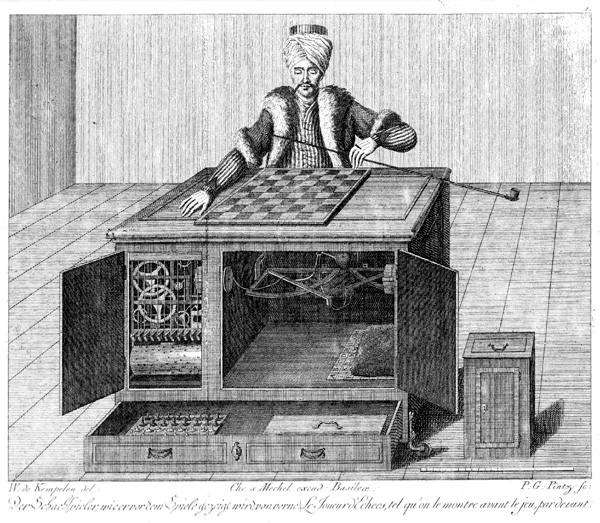
\includegraphics[width=0.7\textwidth]{Turk-open.jpg}
\caption{Engraving of the Turk. This shows the Turk with open doors and the different parts inside of the Turk. Wolfgang von Kempelen may have drawn this picture himself, since he was a talented engraver \cite{theturk}.}
\end{figure}

\paragraph{Advantages with Amazon Mechanical Turk}
There are several advantages of using AMT for conducting behavioural research surveys. Amazon Mechanical Turk enables the opportunity to reach out to a wide audience, since it provides access to a large subject pool \cite{AMT}. When conducting a survey or other research for example in connection with school projects etc., you seldom have access to a large subject pool. Usually you may get your friends to contribute, and maybe some other people going to the same school or a few people living in the same place. The results of this survey or research will most likely be reflected by lack of diversity. If you use Amazon Mechanical Turk instead, you get yet another advantage; subject pool diversity. The workers on Mechanical Turk are spread all over the world, and have different backgrounds. They have different religions, ethnicity, languages, different positions in society (economical), and age. The one last advantage with Mechanical Turk worth mentioning is that you get access to all the aspects mentioned above at a low cost. The workers are willing to take jobs and perform task for relatively low pay \cite{AMT}.

\paragraph{Financial Incentives} 
Some concerns regarding the financial incentives are brought up in connection with Mechanical Turk (MTurk). One question is whether or not lower pay result in lower quality in the work conducted by the workers. It is important to have knowledge about the relationship between how good the workers perform, and the financial incentives given to them \cite{incentivesAmt}. Research done by Horton and Chilton \cite{amtpay} shows that the least amount of pay a worker is willing to accept for a task on MTurk is \$1.38 per hour, and they refer to this amount as the \emph{reservation wage}. 
\subparagraph{}
The article "Analyzing the Amazon Mechanical Turk Marketplace" \cite{averagepay} written by Panagiotis G. Ipeirotis in December 2010 shows that the effective hourly wage on MTurk is \$4.80. This is calculated based on some observations, and also on some assumptions. What they observed was that the median arrival rate was \$1.040 per day, and that the median completion rate was \$1.155 per day. They then assumed that MTurk acts like an M/M/1 queuing system. Based on these observations and assumptions they used basic queuing theory and calculated that a task worth \$1 is completed with an average of 12.5 minutes. Like mentioned earlier, this results in an effective hourly wage of \$4.80.
\subparagraph{}
Winter and Mason \cite{incentivesAmt} conclude that if you increase the pay, the quantity of participants increases, but the quality of the work done does not increase. They think the reason for this is the \emph{anchoring effect}. The anchoring effect describes that it is common for humans to depend too much on the first information given to them when making decisions \cite{anchoring}. In the case Winter and Mason presents: the workers who get more pay, also assume that the work they are about to conduct is more extensive, and therefore do not get more motivated to perform the work. 

\section{SurveyMonkey}
SurveyMonkey is the world's leading provider of web-based survey solutions \cite{surveymonkeyaboutus}. SurveyMonkey was founded in 1999 by Ryan Finley, and had 15 million users in 2013 \cite{surveymonkeywiki}. Using SurveyMonkey as a tool you are allowed to create your own survey based on templates. To get started with SurveyMonkey and to create surveys you have to register the site, and choose account type after need. The different account types have different prices. The more expensive, the more is included. There are several features available when using SurveyMonkey \cite{surveymonkeyfeatures}. It is easy to create questions, with 15 question types available. You can also add logic to the questions. It is easy to customize the appearance of the survey, with the colors you prefer and so on. Getting responses on the survey is done by sharing an URL, for example on Facebook or in e-mails. When you have gotten answers on your survey, you get the data presented in graphs and charts. You can also export the results in various ways, for example all response data or just individual responses.


\cleardoublepage

\chapter{Facebook Privacy}
\label{chp:defaultprivacysettings} 

In this chapter we are going to look into was kind of privacy settings that exist on Facebook and the history of Facebook's privacy settings. We will also look at and map how the default privacy settings has evolved over time. In addition to this we will look at some of the features introduced by Facebook over the years, and how these features have effected the privacy on Facebook. Finally we will review some of Mark Zuckerberg's  thoughts and comments in regard to Facebook privacy. 


\section{Privacy on Facebook}\label{sec:privacy_on_facebook}

%-dra inn undersøkelse 
%-hva slags type settings som finnes? 

\begin{figure}[h!]
\centering
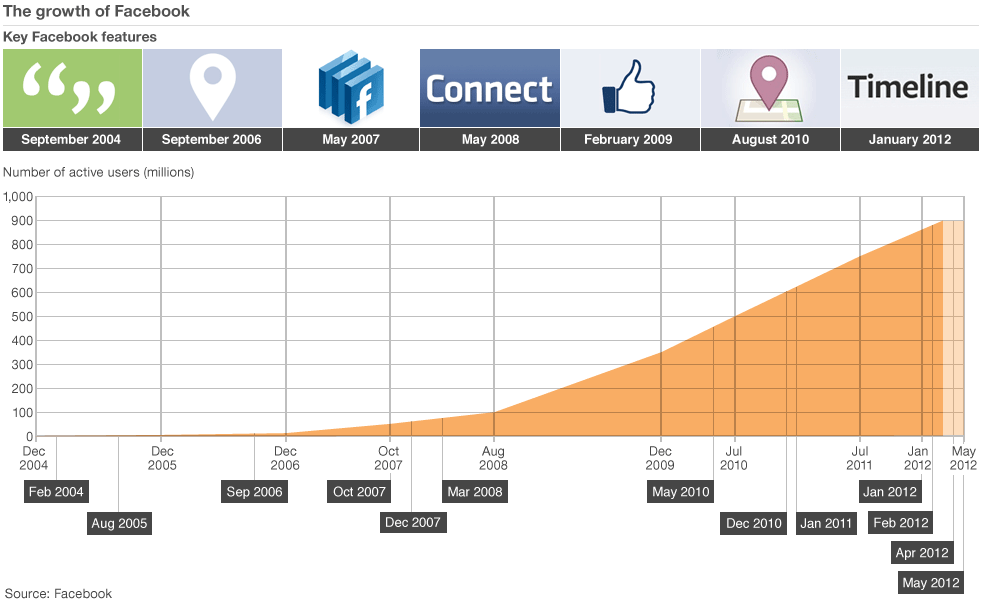
\includegraphics[width=0.8\textwidth]{gowth_of_facebook.png}
\caption[The development of Facebook users and introduction of new features]{\textbf{The development of Facebook users and introduction of new features.} The orange field in the graph shows the increasing number of Facebook users over the years. Key Facebook features are shown over the graph according to when they were introduced \cite{BBCFacebookGrowth}.} 
\label{fig:growth_of_facebook}
\end{figure}

There is no doubt that Facebook has had a remarkable development, both when it comes to number of active users and the development of new features, as shown in \fref{fig:growth_of_facebook}. Along with new users and new features, there has also been made changes to what kind of privacy settings exists and that are needed. 


\subsection{Facebook Settings}
%- kort og hvilke settings som finnes, hva du har muligheten til å endre på



\section{Default Privacy Settings on Facebook}\label{sec:default_privacy_settings}

Facebook has evolved from being a networking site for students attending Harvard to becoming a global phenomenon. Facebook's user interface has gone through several changes over the years, which has brought both joy and frustration to the users. When these changes have been made, there has also been adjustments to the default privacy settings as well \cite{EvoPriv2}. At the beginning, in 2005, when Facebook first was applied outside of Harvard University, the users personal information was only accessible to a users Facebook friends and to people connected to the same network on Facebook \cite{EvoPriv}. This is far from reality today. We will now look into how the default privacy settings on Facebook has developed over since it was first introduced. 


\subsection{Development of Default Privacy Settings}

%- skrive litt mer her, en slags intro
\begin{center}
\begin{table}
\caption{\label{tab:dps}Changes in the default privacy settings on Facebook from 2005 until today. \cite{EvoPriv,PrivTimeline}}
    \begin{tabular}{ | l | p{9cm} |}
    \hline
    \textbf{Year} & \textbf{Default Privacy Settings} \\ 
    \hline
    2005 & Personal information (e.g., name and profile picture) is 	only visible to specific groups specified in your privacy 			settings.\\ 
    \hline
    2006 & The only information displayed in your profile is your 		school and specified local area. \\ 
    \hline
    2007 & Name, name of school (network) and profile picture 			(thumbnail) is available to all Facebook users.\\
    \hline
    November 2009 & Name, profile picture and demographics is 			available and searchable to the entire Internet. In addition to 	this, list of friends are visible to all Facebook users.\\
	\hline
    December 2009 & Your name, profile picture, list of friends, 		pages you are fan of, demographics and likes are available for 		the entire Internet.\\
    \hline
    April 2010 & The entire Internet can see everything, except 		wall posts that are limited to friends and photos that are 			limited to your network. \\
    \hline
    2011 &  \\
    \hline
    2012 & \\
    \hline
    November 2013 & The entire Internet can see everything, except posts you've been tagged in on your timeline and others posts on your timeline, which are limited to friends of friends. \\ 
    \hline
    \end{tabular}
   \end{table}
\end{center}

%- utdype tabellen 

The main changes to the default privacy settings are emphasized in \tref{tab:dps}. 

% utdype mer, se kilde
Secure browsing became default in July 2013. Since 2011 users have been able to turn on secure browsing.  \cite{secureBrowsing}

\subsection{Default Settings 2013}
\label{subsec:default2013}

To examine the default settings on Facebook anno 2013, we created a new Facebook profile, so we could see how the settings were as default. \fref{fig:security2013}, \fref{fig:privacy2013}, \fref{fig:timelineandtagging2013} and \fref{fig:apps2013} shows the outline of the different settings without any alterations, in other words the default settings. 

\fref{fig:security2013} shows how the default security settings look like in November 2013. As we can see from the Figure, secure browsing is enabled by default. 

\begin{figure}[h!]
\centering
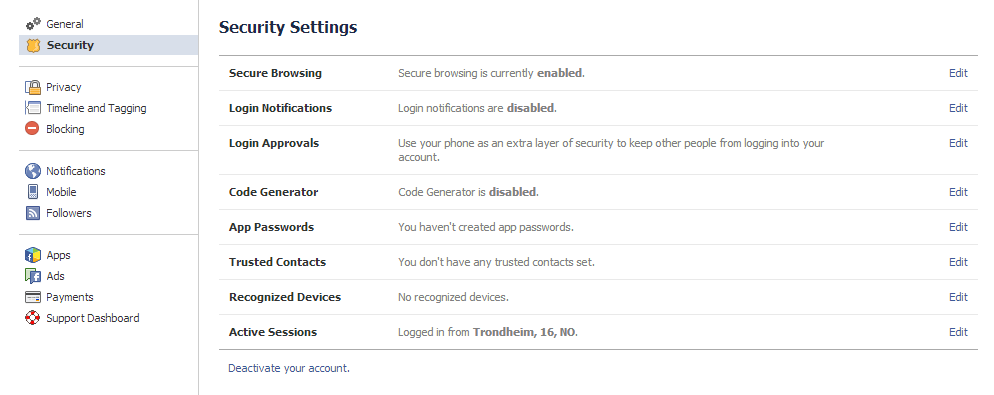
\includegraphics[width=1\textwidth]{default_nov_2013_security.png}
\caption[Default security settings on Facebook November 2013]{\textbf{Default security settings on Facebook November 2013}. This Figure shows the default security settings on Facebook in November 2013.} 
\label{fig:security2013}
\end{figure}

\begin{figure}[h!]
\centering
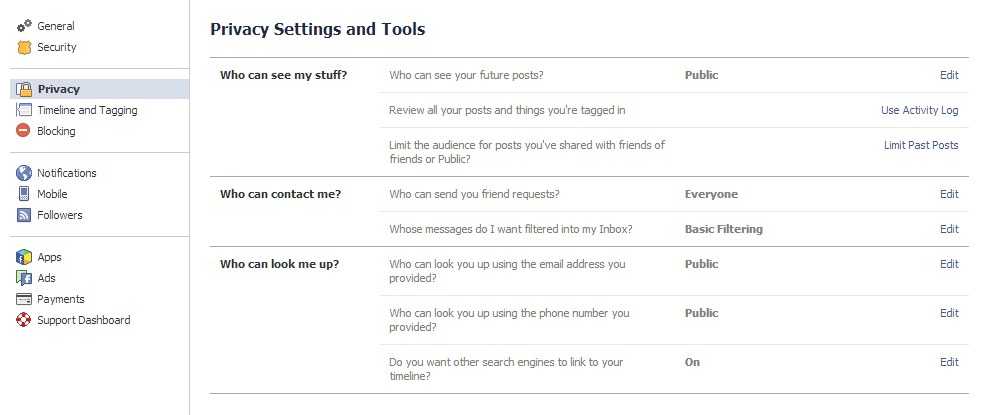
\includegraphics[width=1\textwidth]{default_nov_2013_privacy.png}
\caption[Default privacy settings on Facebook November 2013]{\textbf{Default privacy settings on Facebook November 2013}. This Figure shows the default privacy settings on Facebook in November 2013.} 
\label{fig:privacy2013}
\end{figure}

\begin{figure}[h!]
\centering
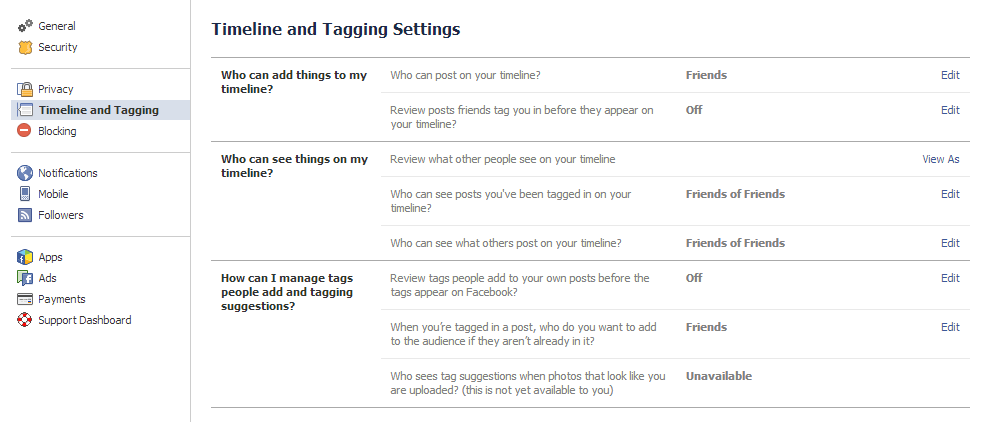
\includegraphics[width=1\textwidth]{default_nov_2013_timelineandtagging.png}
\caption[Default settings for timeline and tagging on Facebook November 2013]{\textbf{Default settings for timeline and tagging on Facebook November 2013}. This Figure shows the default settings for timeline and tagging on Facebook in November 2013.} 
\label{fig:timelineandtagging2013}
\end{figure}

\begin{figure}[h!]
\centering
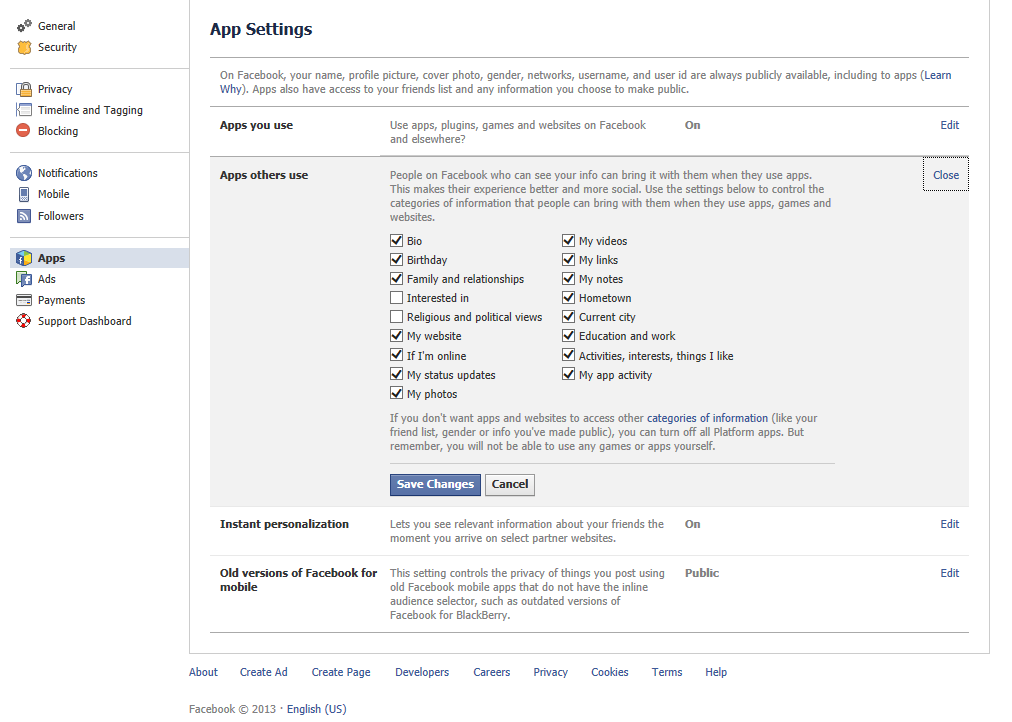
\includegraphics[width=1\textwidth]{default_nov_2013_apps.png}
\caption[Default settings for apps on Facebook November 2013]{\textbf{Default  settings for apps on Facebook November 2013}. This Figure shows the default settings for applications on Facebook in November 2013.} 
\label{fig:apps2013}
\end{figure}

\fref{fig:privacy2013} shows the default privacy settings in November 2013.  \textit{"Who can see your future posts?"} is set to \textit{Public}, which means everyone can view you posts. \textit{"Who can send you friend requests?"} is set to \textit{Everyone}. \textit{"Who can look you up using the email address you provided?"} and \textit{"Who can look you up using the phone number you provided?"} is set to \textit{Public}, which means it is easier for people to find you on Facebook if they know you email or phone number. The setting \textit{"Do you want other search engines to link to your timeline?"} is turned \textit{on}. This means that for example if you google a person, the Facebook profile will appear in the search. To summarize, the privacy settings are \textit{as public as they can get} by default. 

\fref{fig:timelineandtagging2013} shows the default settings for timeline and tagging of Facebook in November 2013. \textit{"Who can post on your timeline?"} is set to \textit{Friends}, which means that only Facebook friends can add things to your timeline. \textit{"Review posts friends tag you in before they appear on your timeline?" }is set to\textit{ off}. This means when friends tags you in something, it will appear on your timeline before you have had a chance to review it. In most cases this is probably fine, but it may occur that a Facebook friends tag you in something you would not prefer to have displayed on your timeline. In these cases it would be desirable to have the review-setting turned on. \textit{"Who can see posts you've been tagged in on your timeline?"} and \textit{"Who can see that others post on your timeline?"} is set to \textit{Friends of Friends}. In contrary to those who can post on your timeline, which are friends, friends of friends are able to view the content added to your timeline. If you have many friends on Facebook, and these friends have many friends each, the audience for posts are suddenly extremely large. 

\paragraph{Default settings does not preserve privacy} It is safe to conclude that the default privacy settings on Facebook anno 2013 is far too public. Unless there are conducted changes to the privacy settings, the timeline will be publicly available, with the exception of posts you've been tagged in and other's posts on your timeline which is "only" visible to friends, and friends of friends. 

\subsection{Default Settings for Teens}

\begin{figure}[h!]
\centering
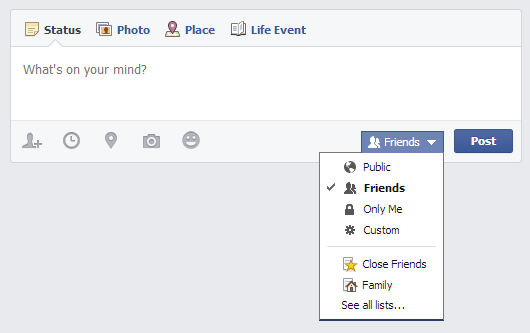
\includegraphics[width=0.8\textwidth]{new_post.png}
\caption[Choosing who can see a status update.]{\textbf{Choosing who can see a status update}. When posting a new post the user can choose the audience the post will be visible to. This can either be "public", "friends", "only me" or "custom".} 
\label{fig:newPost}
\end{figure}

\begin{figure}[h!]
\centering
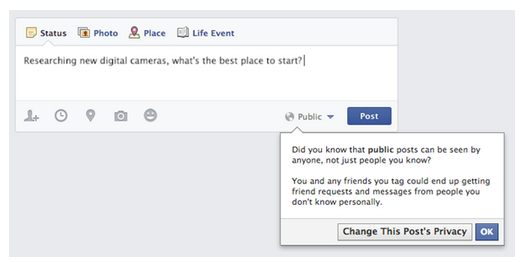
\includegraphics[width=0.8\textwidth]{teensSharePost.png}
\caption[The message shown to teens when posting to the public for the first time]{\textbf{The message shown to teens when posting to the public for the first time.} After the first time they post to the public the message in \fref{fig:sharePost} is shown \cite{defaultTeens}.} 
\label{fig:teensSharePost}
\end{figure}

\begin{figure}[h!]
\centering

\includegraphics[width=0.8\textwidth]{sharePost.png}
\caption [The message shown to teens when posting to the public, except for the first time]{\textbf{The message shown to teens when posting to the public, except for the first time.} The first time they post to the public the message in \fref{fig:teensSharePost} is shown \cite{defaultTeens}.} 
\label{fig:sharePost}
\end{figure}

Each time a user on Facebook share a status update, the user chooses who the post is visible to, see \fref{fig:newPost}. The change you make will remain the same in future posts, unless you decide to change it. Up until today the default audience is set to "public", but for teens between 13-17 years, it has been "friends of friends". On October 16th Facebook announced to change the default setting for teens \cite{defaultTeens}. Now the initial audience for posts are "friends". Teens can later change this to "public", this was not a option before. Teens are active users of social media, and have want to be heard, either it is political engagement or an opinion on a movie. Further Facebook allows teens to turn on Follow, by doing this their public posts will show up in people's news feeds. Facebook designed these changes to improve the facebook experience for young people. In \cite{defaultTeens} Facebook also makes it clear that they take the safety of teens very seriously, and therefore have created a more extensive warning message, shown in  \fref{fig:teensSharePost}. This message appears when a teen changes the audience for their post. If they continue to post to the public, they will will get an additional reminder message, as shown in  \fref{fig:sharePost}.

\section{Facebook Features - Impact on your Privacy}\label{sec:facebook_features}


\subsection{News Feed}
\paragraph{}
"Somehow we missed this point with News Feed and Mini-Feed and we didn't build in the proper privacy controls right away. This was a big mistake on our part, and I'm sorry for it." \cite{FacebookStoryInceptionToIsp}

\subsection{Facebook Platform - Apps}


\subsection{Beacon}
%-Det må fylles ut mer her!

\paragraph{}
At the end of 2007 Facebook launched the feature called Beacon. Beacon was created to help users easily share information from other websites with their Facebook friends \cite{BeaconWebsites}. Beacon was a key part of the Facebook Ads system. The aim was to connect businesses and users and create a more targeted advertising towards the users. 

When Beacon was launched it had 44 partner site, among these are Live Nation, fandango.com, Trip Advisor, STA travel, eBay, the Knot and Zappos.com. According to the Facebook announcement \cite{BeaconWebsites} these websites could determine which actions was most relevant and appropriate for a user to share on Facebook. This could be anything from watching a video, a new high score on an online game, posting an item for sale or completing a online purchase. When a user, that is logged on to Facebook, enters a website that is part of Beacon, they will receive a message asking whether they would like to share their actions on Facebook. If a users agrees, the users actions on that page will be shown in their news feed or mini feed and shared with their friends.  

Beacon received a lot of attention and privacy concerns. Some websites posted to Facebook without asking the users if they want to share the information first. Beacon is a very short piece of code provided by Facebook. The participating websites implement this code on the actions that they would like people to share. An example described in \cite{beaconMarketsPerspective} is with the blog page TypePad. The user have the opportunity to chose whether Beacon should be turned on or not. When creating a post and publishing it the user receives a small pop-up window in the lower right corner stating that you are now sharing this information with Facebook. The pop-up allow you to answer no, but here you have to be quick, the window is not visible very long. When entering Facebook a message is shown at the top of the users wall. Telling the users that a website have shared information with Facebook. You then have the opportunity to go through and select weather that website is allowed to share at all, to just friends of to the public.  

But not all websites have created an option for the users to themselves choose to opt-in. And pushes to Facebook without notifying the users or lets the users select themselves that they want to share it. An much used example of this is a man buying and engagement ring online and the website posts on Facebook. Before the guy have the time to remove it, both friends and family and also the coming fiancée have seen it. So much for the surprise engagement.  
This is unfortunate for the users, but also for the companies using Beacon, it puts them in a negative light. 

Another problem is that Beacon only checked that a user was logged on Facebook. When several people use one computer it could create problems, since Beacon was machine specific. One family member, the mother, could be logged on while her 10 year old son plays an online game, and manages to make a new high score. This high score will then be posted in the newsfeed on the mothers Facebook profile, and shown to the mothers friends.  Beacon only checks that there is a valid Facebook cookie on the machine and then pushes the content to that Facebook user, without any validation. 

\paragraph{}
In a blog post, Mark Zuckerberg apologized for the way the feature was created and for the handling of the complaints in hindsight. 
\cite{Beacon} 

\subsection{Facebook Connect - "Log in with Facebook"}
From may 2008 users had the ability to connect and log in to other web pages via Facebook, "log in with Facebook" 


\subsection{Timeline}
As mentioned in section \ref{sec:facebookhistory} in Chapter 1, the Facebook timeline was introduced in December 2011 \cite{EvolutionOfFacebook}. This feature made the entire history of the users visible: your posts, posts by others, likes, photos, links, pages liked, comments and other things that you have shared on Facebook. The timeline showed much more than the old profile did, and it was far more visual \cite{timeline}. On the top of your timeline it is room for a big photo. This photo is called a \emph{cover photo}. Cover photos are publicly available, and it is not possible to change the settings for them. You can of course choose which photo you want as your cover photo, or just choose not to have a photo there at all. When scrolling down your timeline , you'll see photos, posts etc. and different events in your life in order of when they happend in time \cite{timeline}. You can look at it as the story of your life. You get the opportunity to "go back in time" and fill in the blanks. If you want to emphasize, for example an event or a photo, you can highlight it with a star, or on the other hand, if you want to hide something from the timeline you can also do so. 

\paragraph{Privacy concerns regarding Facebook timeline}
When timeline was introduced many people became overwhelmed by the changes, and felt they lost control over their privacy. When you agreed to start using timeline, you got a certain period of time to review and edit your timeline before making it public. This gave the users the opportunity to clean up their timeline before everyone else could view the content of it. Cleaning up the timeline can be done using something called the "Activity Log" \cite{activitylog}, which is shown in \fref{fig:activitylog}. The activity log is basically a list over everything ever done in connection with you on Facebook, either done by you or by others. The activity log also makes it easy to view and change the audience for the different "activities". If you are an active user of Facebook, reviewing the whole activity log can be very time consuming. 

\begin{figure}[h!]
\centering
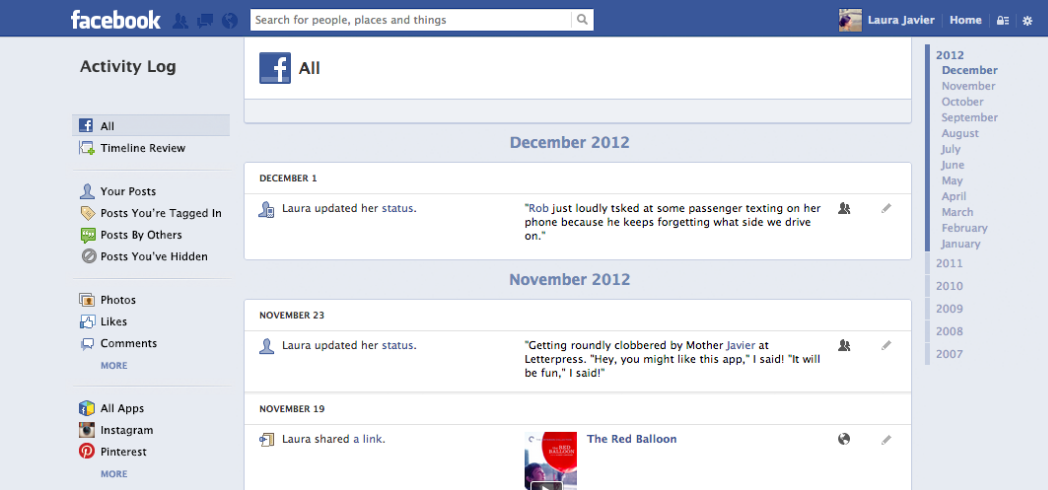
\includegraphics[width=1\textwidth]{activity_log.png}
\caption [Example of an activity log on Facebook.]{\textbf{Example of an activity log on Facebook}. On the left side you see types of content. If you want to view for example "Posts by others" you can do so by clicking on it. To the right you see a list of the years and months. You can click on which year or month you want, and review the activity from that year/month \cite{activitylog}} 
\label{fig:activitylog}
\end{figure}

\paragraph{}
The introduction of timeline was not in itself a privacy breach since you had, and still have, the opportunity to decide what you want to be visible on it, and what you want to hide. On the other hand, there are people who are extra exposed when Facebook introduced new major changes, like the timeline. Lets refer back to section \ref{sec:relatedwork_facebookprivacy} in Chapter \ref{chp:relatedwork}, where we highlighted some of the findings from the survey addressed in the paper "Facebook privacy settings; Who cares?" by danah boyd and Eszter Hargittai \cite{whocares}. boyd and Hargittai concluded their paper, based on their survey and findings, that experience and Internet skill is important to take into account in regard to how people handle their privacy settings on Facebook. Since familiarity with technology plays a role in how people handle their Facebook privacy settings, one can assume that the least skilled people get more exposed when Facebook changes the outline of the default privacy settings. 
This can be seen in the context with the introduction of the timeline. The least skilled users of Facebook that perhaps do not know how to change their privacy settings, probably was left extra exposed when the timeline was introduced and their timeline may have shown, and may still show, more than they actually would prefer. 

There also exits privacy settings connected to you timeline under "Timeline and tagging" in your settings on Facebook. You can regulate who can add things to your timeline, and who can see things on your timeline. Under "Privacy" you can also regulate who can see your future posts. 

\subsection{Graph Search}


\subsection{Facebook Removes Search Privacy Setting}
Facebook announced October 11 that they will remove the setting that has made it possible for Facebooks users to hide from the ability to be looked up on the Internet\cite{searchSetting}. It was only the users that have not used the setting "who can look up my timeline by name" in December by last year that was affected by the change. Facebook explains the removal of the feature by it being outdated, and that there are several others ways to find a persons time line. They argue that it can be confusing for the user when they try to look up someone and do not find them. Mark Zuckerberg said that a users should do things they want to keep secret.

(sånn jeg ser det så er det jo fult mulig å søke opp hvem som helt på faceboko sin egen søkefunksjon, det betyr jo ikke ta jeg ønsker å være søkbar på google. 


\section{Zuckerberg's Thoughts}

\paragraph{}
Zuckerberg ones said this about Facebook in a one of his meetings: "I mean, one way to look at the goal of the site is to increase people’s understanding of the world around them, to increase their information supply," he said. "The way you do that best is by having people share as much information as they are comfortable with. The way you make people comfortable is by giving them control over exactly who can see what" \cite{MeMedia}.

\paragraph{}
This comment from Zuckerberg brings out his thoughts around the privacy issues. He wants the users of Facebook to be comfortable with sharing information, and give them this confidence by giving them control. In general the privacy settings and restrictions that Facebook has have protected the users. They can easily change the setting and decide who can see what. Zuckerburg firmly means that you should not post comments or pictures of things you do not want anybody else to see. And if a user does so, the user has to take the blame for it, not Facebook. Zuckerberg was once asked about pictures put on Facebook of students drinking at an East Coast college, which led to some students being expelled. His answer to this question was: "First of all, it's pretty stupid if you put up pictures of you doing drugs on Facebook. I think that that's just sort of the deviant behavior on the very far end of the distribution. I bet that those kids do not post pictures of them doing drugs on Facebook anymore." He added that he meant this was a "pretty shitty way to learn that" \cite{MeMedia}.

\paragraph{}






\paragraph{}
Mark Zuckerberg wrote this in a letter to possible investors \cite{LetterToInvestors};

\textit{Facebook was not originally created to be a company. It was built to accomplish a social mission - to make the world more open and connected.}

\textit{People sharing more - even if just with their close friends or families - creates a more open culture and leads to a better understanding of the lives and perspectives of others. We believe that this creates a greater number of stronger relationships between people, and that it helps people get exposed to a greater number of diverse perspectives.}

\textit{By helping people form these connections, we hope to rewire the way people spread and consume information. We think the world's information infrastructure should resemble the social graph - a network built from the bottom up or peer-to-peer, rather than the monolithic, top-down structure that has existed to date. We also believe that giving people control over what they share is a fundamental principle of this rewiring.}

\textit{We think a more open and connected world will help create a stronger economy with more authentic businesses that build better products and services.}

\paragraph{Skal vi ha med det her?}
User control became a hot topic already in 2006. There had been reported that sex- offenders was using social networks to pick out their victims. MySpace found out that several teenagers had been assaulted by people they meet at their web page. Facebook also received some negative mention in the press. Numerous times the campus police had to shut down big parties announced on Facebook. In 2005 a student a Fisher college was expelled after posting this comment about the schools police officer "needs to be eliminated" \cite{MeMedia}.

\cleardoublepage

\chapter{Construction of the Survey}
\label{chp:amtsurvey} 

To be able to map to what extent people care, and are aware, of their Facebook settings, regarding privacy, security and interdependent privacy, we designed and distributed a survey. The complete survey can be found in Appendix \ref{chp:appendixA}. The survey addressed the different settings available on Facebook, and awareness regarding Facebook applications and knowledge about interdependent privacy. For the design of the survey we utilized SurveyMonkey, which provide a web-based survey solution (see section \ref{sec:sm}). We distributed the survey on two platforms, namely Amazon Mechanical Turk (MTurk) and Facebook. Amazon Mechanical Turk is a Internet marketplace where human intelligence is utilized to perform various tasks \cite{amazonweb}. For more information about Amazon Mechanical Turk, see section \ref{sec:amt}. To reach out to an even larger audience, we also posted the survey-link on our private Facebook pages. In this chapter we will describe how we designed the survey, and how it was structured, and how we distributed our survey.


\subsubsection{Constructing the Survey.}
There is not much research on the area of interdependent privacy. When designing the questions to our survey, we wanted to be able to create an image of people's Facebook usage, how they set their settings, how much they knew and cared about their privacy, and to what extent their privacy was dependent on other users. We quickly chose to use MTurk as a platform for distributing the survey, because we wanted to create an image of the average Facebook user, as well as getting a high diversity among the respondents (different countries, age, education etc.). Previous research shows positive results with the use of MTurk \cite{expectations,incentivesAmt}. 

\paragraph{}
We started implementing the survey inside the survey template provided by MTurk, but after some consideration, we found that MTurk did not fulfil our requirements for design. We therefore chose to implement the survey using SurveyMonkey instead. During the creation of the survey, we thought that it would be better to include some extra questions, rather than leaving some out. This was to assure that we got all the information we would need in order to perform our analysis. When the survey first was distributed, we were no longer able to edit the questions. We therefore chose to include questions, not only regarding privacy and interdependent privacy, but also other aspects of Facebook usage. Like for instance some questions about security settings, usage, personal experience in regard to photos and comment sharing.

\section{Design}
MTurk offers a template for creating surveys, and this template uses HTML-code. It is simple, but requires more work and knowledge from the requester. We found the template to not be very user friendly, and it did not offer many design options. Our survey consisted of many questions, and some of them had follow-up questions requiring text answers. It was then desirable to separate these into two different pages, as we did not want the respondents to have their answers affected by the next question. It required more of the respondent to write a text answer, so to avoid them answering based on the next question we separated the questions onto different pages. For example, we had one question asking whether or not the use of Facebook has lead to any uncomfortable situations. If the user answered "Yes", a follow-up question asking to describe the situation that occurred would appear. If the user answered "No" the follow-up question would be skipped. If the user had seen the follow-up question, he/she may not be bothered to answer yes even though this may have been the truthful answer. We did not find an easy solution to implement this design feature in MTurk, so we looked for other options. In addition to providing their own "Survey"-template, MTurk also provides a "Survey Link"-template. This means that you can create the survey somewhere else, and link to it in MTurk. We chose the latter, and used SurveyMonkey to create our survey. SurveyMonkey provided us with the tools and features necessary to design our survey as desired. 

\subsubsection{Features we used in SurveyMonkey.}
SurveyMonkey offers several features, and has an intuitive and simple user interface. It was easy to implement the questions, and separate them into different pages, which was of high value to us. SurveyMonkey offers the ability to customize the appearance (color/theme, layout, etc.) of the survey to a higher extent than MTurk. We included a picture of the university logo, to emphasize the seriousness of the survey, as shown in \fref{fig:frontpage}. SurveyMonkey also offers many different types of question forms, like multiple choice, text box, matrix and drop-down menus, and restrictions on the questions. Some of the restrictions that we used was to limit the amount of characters in the text boxes, to avoid too long answers. We also made almost all questions mandatory, meaning that the respondents had to answer them before being able to move on to the next question. As mentioned we divided the questions on to several different pages. In addition to the advantages already mentioned, it would also give the respondents the impression that the survey is shorter. Each page has a title at the top, grouping the different areas. A progress bar was added to the bottom, showing in percent how far into the survey the respondent was at any time. This gave a good overview, and the user got a feeling of how much was left of the survey. We chose to use these features to avoid overwhelming the respondents with too many questions at a time. 

SurveyMonkey offers a great user interface also when it comes to reviewing the answers. It is possible to see graphs showing the distribution of answers to all of the questions, as well as individual answers. SurveyMonkey also offers features as filtering and comparing, which made the analysis a lot easier, especially when having a large number of respondents. 

\section{Survey Structure} 

\begin{figure}[t]
\centering
\fbox{

\includegraphics[width=1\textwidth]{firstpagesurvey.png} }
\caption[Front page of the survey]{\textbf{Front page of the survey.}} 
\label{fig:frontpage}
\end{figure}

The first page seen when taking the survey, was an introduction page that shortly explained what the survey was about, and its purpose. This page emphasized the seriousness of the survey. When people saw that it was a research survey carried out by master students at an university, we believed people would answer in a serious manner. The front page also included the requirements for taking the survey, and a short explanation on where to find answers requested in some of the questions. This is shown in \fref{fig:frontpage}. As mentioned earlier, we divided the questions into different areas, and we will now go through each area emphasizing and elaborating the questions we considered most relevant and important. 
 

\subsection{Facebook Usage}
Following the first page, was a single page about Facebook usage. This page included questions about sign-up year, how often they checked their Facebook page, and number of friends. 

\subsection{Facebook Privacy: Settings}
This was a part of the survey where the users needed to be logged into their main account on Facebook in order to check how their privacy settings looked. The questions were taken directly from the "Privacy"-settings and "Timeline and tagging"-settings on Facebook. We divided these questions on to 4 different pages. Before we started asking about specific settings, we asked the users how often they had checked their Facebook privacy settings during the last year. The following pages asked for the privacy settings, and the other for the timeline and tagging settings. These questions were straightforward for the user, since all they had to do was to render the settings they had set themselves. This would easily show us how many of the survey participants that actually had checked their settings, and to what extent they had made them more, or less, private than default. At the end we asked the users whether or not they considered changing their settings after having reviewed them. This could make for some interesting observations, and could also give an impression of whether or not the users cared or were aware of the settings. 

\begin{figure}[t]
\centering
\fbox{
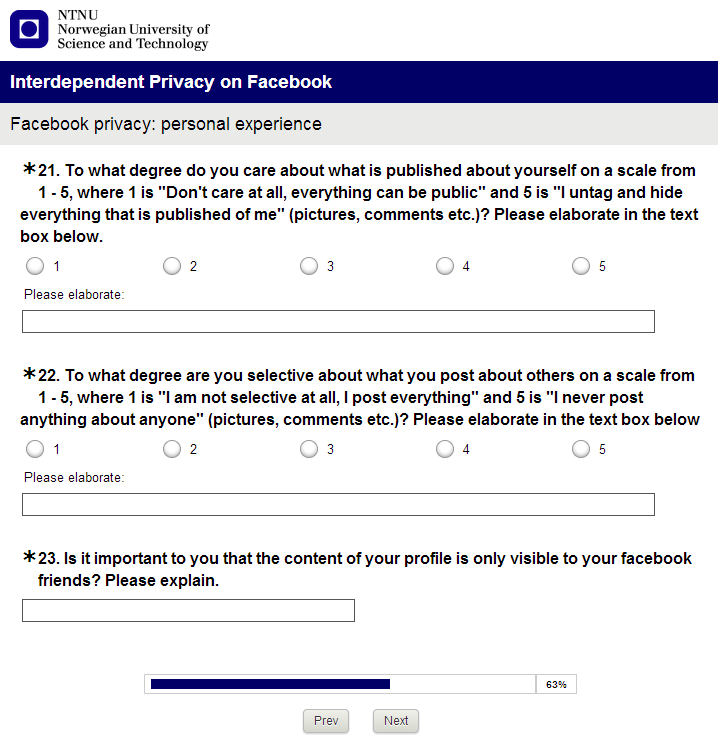
\includegraphics[width=1\textwidth]{page12.png} }
\caption[Question 21 and 22 in the survey concerning personal experience]{\textbf{Question 21 and 22 in the survey concerning personal experience.}} 
\label{fig:page12}
\end{figure}

\subsection{Facebook Privacy: Personal Experience}

This group of questions focused on the users' personal experience with concern to both privacy and interdependent privacy. We asked whether or not the respondents had experienced that their use of Facebook had affected their professional life, or led to any uncomfortable situations. Both of these questions had a follow-up question where the users were asked to describe the situation that occurred. The user would only be sent to the page with the follow-up question if the user answered yes. If the user answered no, the page with the follow-up question would be skipped. 

A big part of Facebook consists of sharing photos and comments with others, we therefore asked the respondents to indicate on a scale from 1 to 5 how much they care about what was published about themselves, and what they publish about others, see \fref{fig:page12}. It was mandatory for the users to give an answer on the scale. We added a text box for the users to elaborate if desired, but this was voluntarily. We received a total of 250 responses on our survey, and 190 of them chose to elaborate. 

\subsection{Facebook Privacy: Apps}

\begin{figure}[t]
\centering
\fbox{
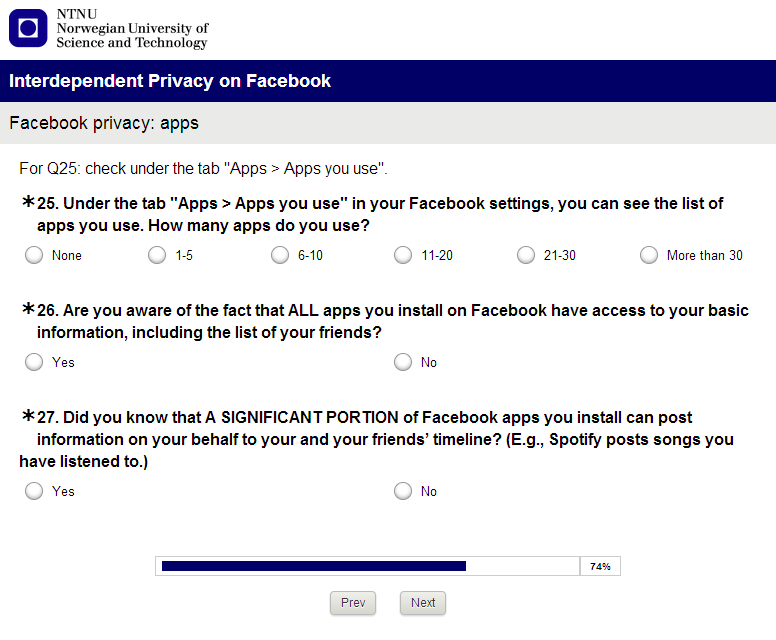
\includegraphics[width=1\textwidth]{page14.png} }
\caption[Question 25, 26 and 27 in the survey concerning Facebook apps]{\textbf{Question 25, 26 and 27 in the survey concerning Facebook apps.}} 
\label{fig:page14}
\end{figure}

\begin{figure}[t]
\centering
\fbox{
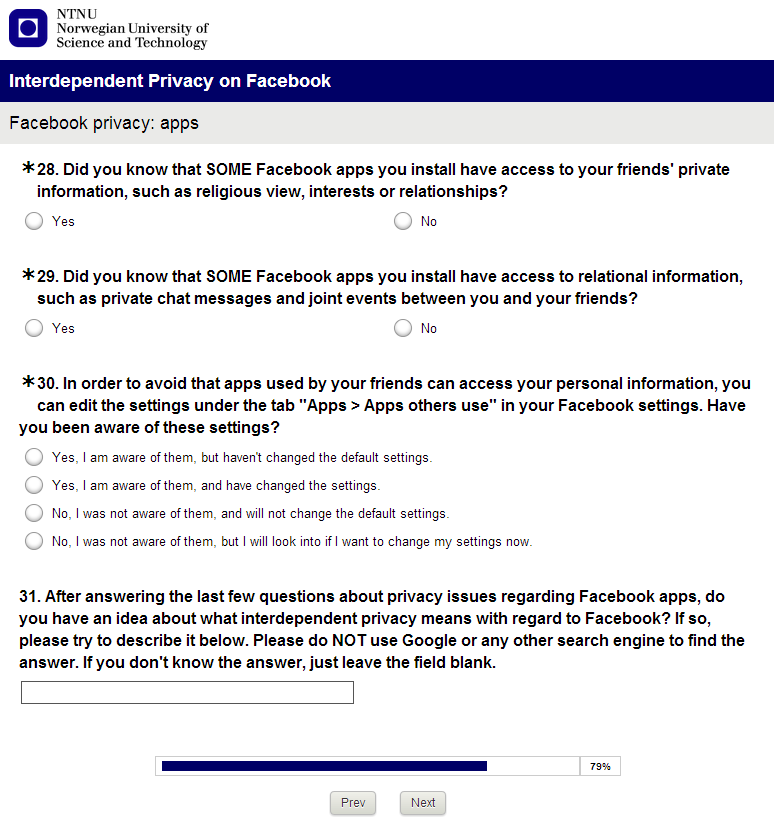
\includegraphics[width=1\textwidth]{page15.png} }
\caption[Question 28, 29, 30 and 31 in the survey concerning Facebook apps]{\textbf{Question 28, 29, 30 and 31 in the survey concerning Facebook apps.}} 
\label{fig:page15}
\end{figure}

This was the part of the survey that concerned interdependent privacy (see section \ref{sec:intpriv}), and also the most important part of our survey. As mentioned earlier, this is a relatively unknown term, so we wanted to find out whether or not the respondents knew the meaning of interdependent privacy. When installing an app on Facebook, it asks for the user's basic information, and often more information about the user and the user's friends. For more detailed information about the app-platform, see subsection \ref{subsec:app}. Question 26, 27, 28 and 29 (see \fref{fig:page14} and \fref{fig:page15}) asked about the user's awareness regarding what kind of information the apps could retrieve. There exists settings directed towards apps on Facebook (see \tref{tab:settings}). Question 25 concerned the number of apps the respondents use. Question 26, 27, 28 and 29 concerned the user's awareness connected to apps permission requests on Facebook. In question 30 (\fref{fig:page15}) we asked the user to look at one of the app settings, "Apps others use". In this setting the user can decide what information they want to make available to apps other people use, in other words, control the categories of information that people can bring with them when they use apps. We did not ask for more specifics about what information they share, because this was not relevant to our research. What was relevant was whether or not they knew it existed, and were aware of what kind of information they shared. We finished this part of the survey with the same question we started it with, if they knew the meaning of interdependent privacy. We wanted to ask again to see if they got a higher understanding of the term after answering questions about apps, and saw how it is all interconnected. 


\subsection{Facebook Security: Settings}
The main focus in this report is on privacy, not security. At the same time, we wanted to ask a few questions regarding Facebook security settings as well. The reason for this was that we wanted to see if there was a connection between strict security settings, and strict privacy settings among the respondents. The questions concerned whether or not the respondents used secure browsing and login notification.

\subsection{Demographics}
In the last part of our survey, we asked for demographic information about the respondents. This to get a hunch of what kind of people had taken the survey. We chose to put the demographics part at the end, rather than at the beginning. We assumed that a respondent's attention span would get lower during the survey, we therefore wanted to put the "easy" questions at the end, since they require less focus. These questions consisted of: gender, age, country, family situation, highest qualification/degree, employment status and income. Although these questions were easy to answer, they were very important to include. When analysing, they are necessary in order to draw comparisons between, for example, age and/or gender. An interesting factor will be to look at where the respondents using MTurk come from.  

\section{Distributing the Survey}


First we created a requester account on MTurk. We did this using an already existing Amazon account. While creating the project (our project contained only one HIT) we filled out the properties shown in \fref{fig:amtedit}. First we had to give a short title and description to describe our HIT to the workers. This is the information that is shown to the workers before they choose to accept, or skip, the HIT. We also had to decide a reward for the workers. We had limited time, and wanted our HIT to be as attractive as possible, and therefore chose to have a higher reward than average. We sat the reward to be \$1.5 per completed assignment. We estimated that it would take approximately 15 minutes to take the survey, and this would give an hourly wage of \$6. We were also asked to set a maximum number of assignments per HIT, this means number of unique answers. We sat this number to be 250. We felt that 250 responses would give us a very good foundation to base our analysis on. MTurk defines a feature that let the requester review the answers, and then choose to either approve or discard them. When discarding an answer, the worker would not get paid. If we did not manually approve the answers, they would automatically be approved after 3 days. We made the HIT available for only 21 days. To get a high quality on the responses, we were advised to use "Master Workers". This is users that have a good reputation from previous work done on MTurk. See section \ref{sec:methodology} for more information about "Master Workers". 

\begin{figure}[t]
\centering
\fbox{
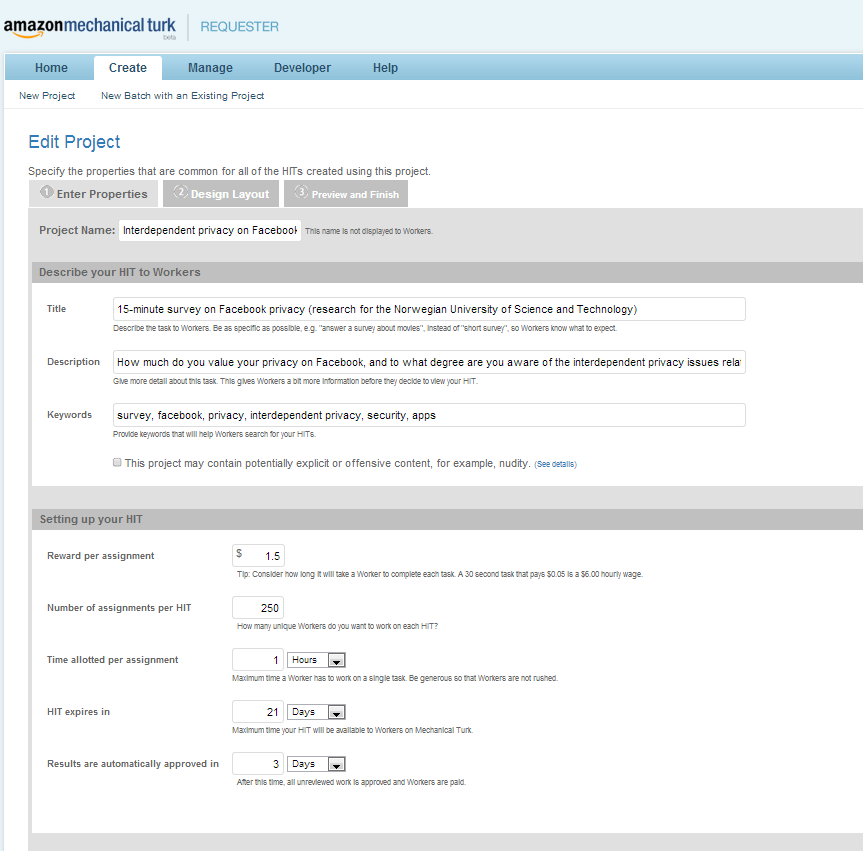
\includegraphics[width=1\textwidth]{amtedit.png} }
\caption[Layout for creating an MTurk project]{\textbf{Layout for creating an MTurk project.}} 
\label{fig:amtedit}
\end{figure}

\begin{figure}[t]
\centering
\fbox{
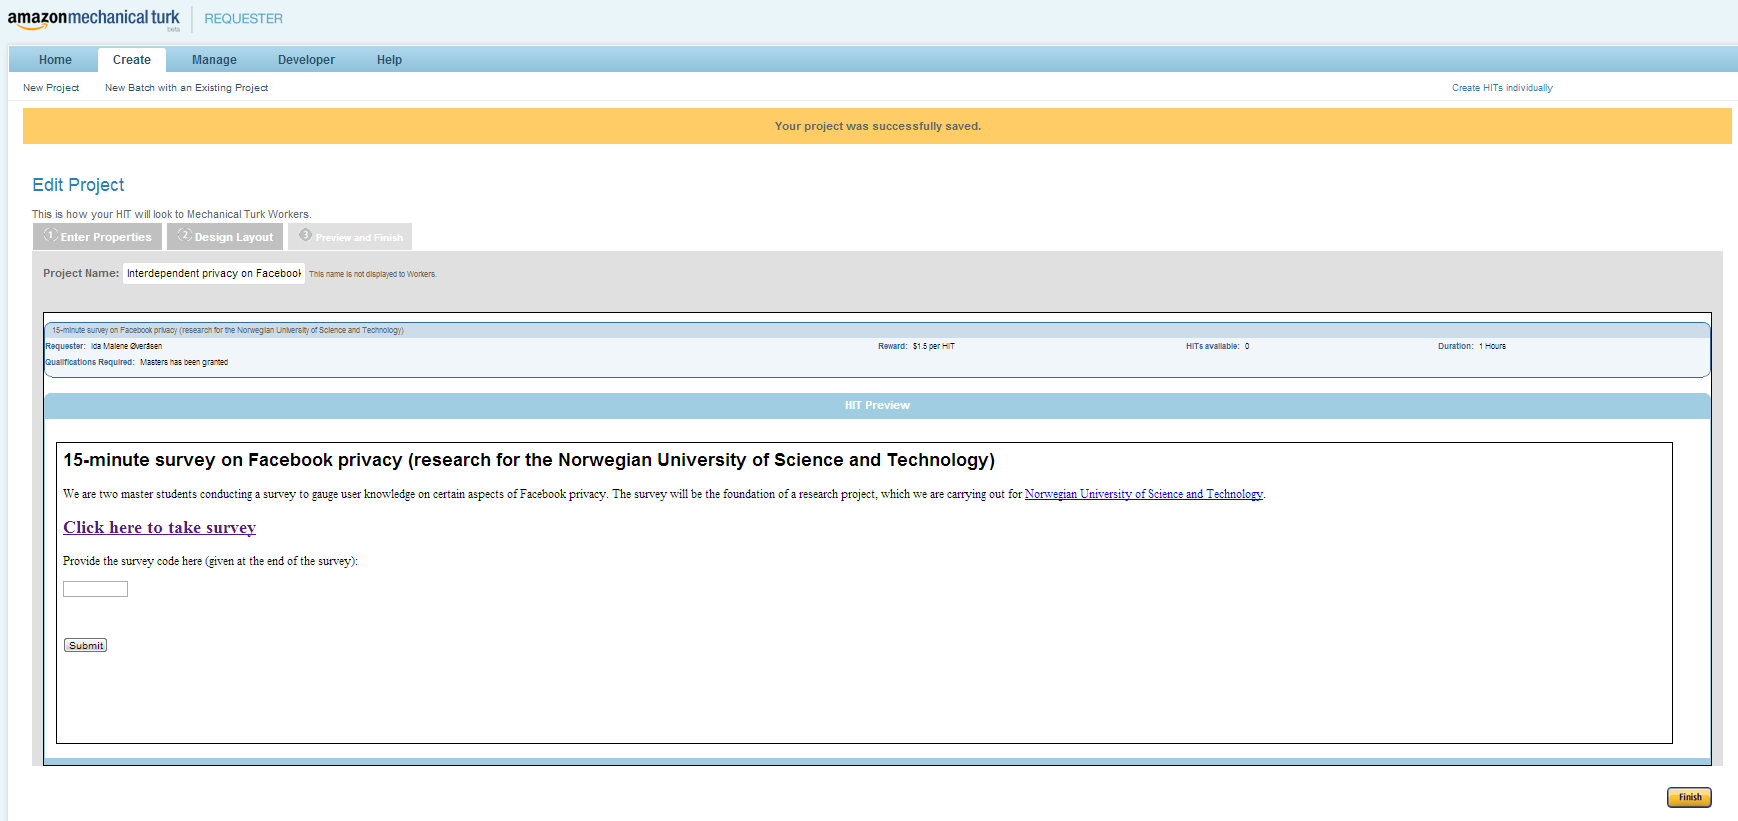
\includegraphics[width=1\textwidth]{amtlayout.png} }
\caption[The design and layout of the survey on MTurk]{\textbf{The design and layout of the survey on MTurk.}} 
\label{fig:amtlayout}
\end{figure}

Next we filled in the "Survey-Link"-template provided by MTurk, and the result of this is shown in \fref{fig:amtlayout}. It contains a title and a short description. In the description we linked to the homepage of the Norwegian University of Science and Technology, to emphasize the seriousness of the survey. In addition it contained the link to the survey on SurveyMonkey, as well as a field for the users to enter a survey code. This code was provided to them after completing the survey, and worked as an assurance for us, so we only paid the people who actually took the survey. To avoid workers cheating with the code (for example getting the code from a fellow MTurk-worker), we changed it several times during the survey's lifetime. 

\begin{figure}[t]
\centering
\fbox{
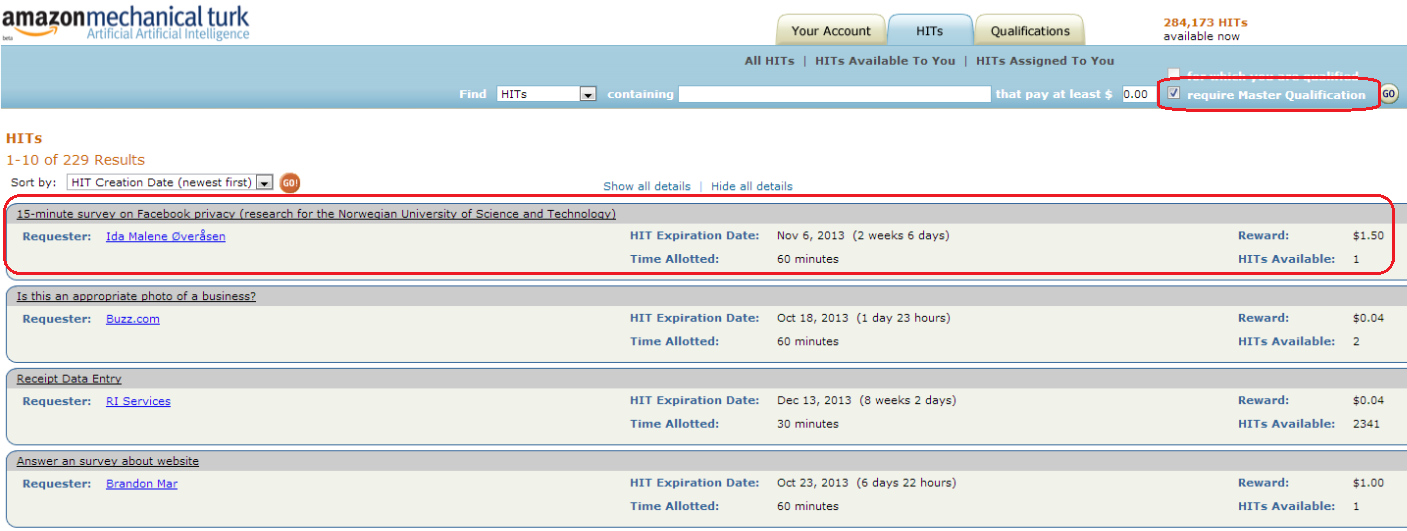
\includegraphics[width=1\textwidth]{hitisout.png} }
\caption[Our HIT is published]{\textbf{Our HIT is published.} This figure shows our HIT in the list of all HITs available that requires "Master Workers".} 
\label{fig:hitout}
\end{figure}

After editing the project, as described above, the HIT was ready to be published. The published HIT is shown in \fref{fig:hitout}. After filtering on HITs requiring "master" qualification, our HIT is shown at the top. 
Once our HIT was out, all we could do were to monitor it (approve or discard answers), and wait for people to respond. 

\begin{figure}[t]
\centering
\fbox{
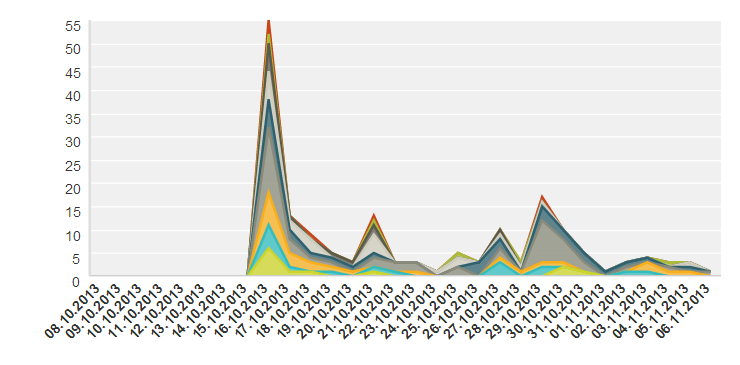
\includegraphics[width=1\textwidth]{answersamt.png} }
\caption[Daily distribution of number of answers from MTurk]{\textbf{Daily distribution of number of answers from MTurk.}} 
\label{fig:answersamt}
\end{figure}

\begin{figure}[t]
\centering
\fbox{
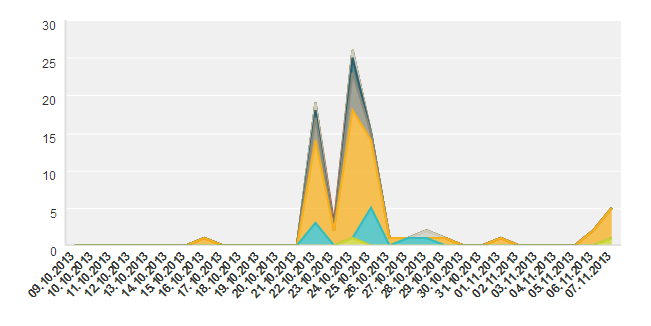
\includegraphics[width=1\textwidth]{answersfacebook.png} }
\caption[Daily distribution of number of answers from Facebook]{\textbf{Daily distribution of number of answers from Facebook.}} 
\label{fig:answersfacebook}
\end{figure}

We mainly wanted to distribute our survey on MTurk, to try it out as a research tool, and because of it's high diversity. But in addition to distributing the survey on MTurk, we decided to also share it with our friends on Facebook. We wanted to reach out to an even wider audience, as well as making our Facebook friends aware of their settings. Most of our Facebook friends mainly consist of fellow students, with high technical knowledge. We were hoping for at least 30 extra respondents as a result from our post on our private Facebook profiles. We received 77 respondents and were amazed with the outcome. A few times during the 3 weeks the survey was out, we pushed our post to the top of our friends' news feeds by commenting on it. Three of our friends even chose to share it on their own Facebook profile. This was probably one of the reasons why we got more answered than expected. We posted the survey on Facebook a few days later than the HIT was published on MTurk.  

\fref{fig:answersamt} and \fref{fig:answersfacebook} shows the daily distribution of number of answers, from MTurk and Facebook respectively. You can see from \fref{fig:answersamt} that we had the highest peak in responses the day it was published on MTurk, with 55 unique answers, and the second day it dropped to 13 answers. The number of responses varied during the rest of the period, as the figure shows. 

\section{Feedback on the Survey}
We got a lot of positive feedback on our survey from our Facebook friends. Many have "liked" it, and many have commented on it. The comments focused mainly on the eye opening aspects of the survey and that it was informative. Some said the survey made them clean-up their settings. Some mentioned that they believed they had good control over their settings, but after taking the survey they realized that this was not the case. Overall, the feedback was very positive. As mentioned above, three of our Facebook friends even chose to share the survey further, meaning that they were pleased with it and thought it was both good and informative. 

Our survey has also been mentioned in forums as, for example, mturkform.com and mturkgrind.com. Most of the comments regarding our survey on these forums were about the time consumed taking the survey and it's complexity. The comments from mturkforum was: \textit{"Time 5 min 35 sec - slow b/c I wanted to learn more about FB privacy..."} and \textit{"Took 8 minutes, light writing but very simple"}.
The comments from mturkgrind was: \textit{"About 5 minutes"} and \textit{"Took 8 minutes, very simple and probably could do it in less time. Light writing"}.






\cleardoublepage

\chapter{Discussion}
\label{chp:discussion} 

\cleardoublepage

\chapter{Conclusion}
\label{chp:conclusion} 

Facebook offers a high variety of settings for the users. The users are given full control over their settings, and can themselves choose whom they want to share information with. As default, most of the settings are set to the most public option available. Facebook states that the users have full control, and that it is the users' responsibility to control the audience for the information they share. They also state that the users should not share information they do not want anyone to see, like posting a picture of someone taking drugs. The most important aspect regarding the Facebook settings is user awareness. If a user is unaware of the existing settings, the settings are of no value to the user. Many of the respondents pointed out that through taking our survey they became aware of settings they did not know existed. In other words, the survey did not only provide us with valuable research data, but was also informative and educational for those who participated.  

When Facebook started as an online environment, available only for Harvard students, privacy was the most important factor. A valid Harvard email-address was required in order to sign up. This provided an assurance that all users of "Thefacebook" were actual people, and this made the threshold of sharing information much lower. In 2005, nothing was publicly available to all Internet users. Most of the information a user shared was visible to a user's network or friends, except name, profile picture, gender and network that was available to all Facebook users. Default settings have become increasingly public with every passing year. In November 2009, significant changes were made to the default settings. Name, profile picture, gender and networks gradually became available to all Internet users. Most of the remaining information (wall posts, photos, likes, birthday) was restricted to friends of friends. There is a theory called "Six degrees of separation" \cite{six}, which states that two people are connected via maximum six steps. This means that when information is shared with friends of friends, the audience is \textit{extremely} large. Major changes to the default settings also took place in April 2010, when everything, except contact information and birthday, was made publicly available to all Internet users. With information becoming increasingly accessible on the Internet, Facebook also announced more settings possible for the users to edit. Today all Internet users can see everything by default, except posts you have been tagged in on your timeline, and posts by others on your timeline, which are limited to friends of friends. There is no doubt that Facebook's default settings have become increasingly public. With this development, the importance of user awareness of existing settings is also becoming more and more crucial. It is essential that the users follow the development, and change the settings according to their personal preferences. 

Along with the development of Facebook, the site has also introduced numerous new features. Some of them have affected the users' privacy more than others, and have received a lot of attention in the media. The single feature that had the most impact on users' privacy was Facebook's introduction of applications. 
The main reason that apps affect a user's privacy is because of the information apps retrieve. What kind of information apps requests to access is very often unclear to the user. When a user installs an app on Facebook, the app shows the user a list of permissions they request to access. These permissions often expand beyond the basic information, such as asking to post on a user's behalf, and sometimes asks access to relational information (this may include private chat messages). These requests often ask for permissions that go against the user's privacy settings, and this leads to a user sharing information that was intended to be private. Our research shows that there has been a change in how the permission requests are shown to the user. In 2011 there was a separate page displaying the permission requests. Today Facebook has introduced the App Center, where the permission requests are shown in small letters on the side of the page, not very visible to the user. Research done on the permissions page in 2011 showed that it should be more clear to the user when they approved permission request that stride against their initial privacy settings. When we look at the permission page today, Facebook have done the opposite. There is less focus on the permissions, and more on the app in general.  
There is no doubt that Facebook has become a far more public and open platform, and promotes the idea of sharing. Facebook always wants to customize all information, adds, apps and news feed-posts, for the users in accordance with their preferences.

User awareness of settings available on Facebook is extremely important. The majority of all the respondents that took our survey stated that they check their Facebook settings to some degree. Most of them, almost half of the respondents, stated that they check their settings 3-6 times a year. On the other hand, only 12\% stated that they had not checked their settings during the past year, but they must have done so at some point, since their settings differed from the default settings. We found a contrast between the ones that seldom check their settings, and the ones that frequently check their settings. Initially, we 
thought that the ones that frequently check their Facebook settings, have more knowledge of the settings that exist, both the privacy/security settings and the settings regarding apps, as well as being more active users. This assumption turned out to be correct. The difference between the ones that check only rarely and those that check frequently was not immense, but large enough to divide these groups. The ones that frequently checked had more private/secure settings in all areas. These users were on average almost 10 years younger than the ones who only checked rarely. This might be because of the hi-tech world that today's young generation have grown up in. The elderly generation does not have the same technological knowledge or insight. One reason why they are on Facebook is that Facebook provides them with the opportunity to stay in touch with old friends and relatives. Several of our respondents stated that they have created a Facebook profile for one single reason: stay in touch with their younger family members. 

Those who checked their settings frequently were also more aware of the permissions apps request, than those who seldom check. There was also a difference when we looked at those who had many apps and those with few apps connected to their Facebook account. We assumed that those with few apps connected had more knowledge of the permission requests. When knowing how much information an app can access, one would think a user would be careful connecting apps to their Facebook account. The number of respondents who were aware of the permissions apps request was higher for the ones having few apps connected to their Facebook account. Even though there was a higher level of knowledge for those with few apps than for those with many apps, the overall level of knowledge of these permissions were low. We think that many users know that the applications may access information, and therefore refrain from installing any apps, in other words just ignore everything regarding apps. But what one might forget is that even though some individuals refrain from installing apps, their friends might not share the same view. For example, although Alice chooses to refrain from everything regarding apps, Alice's Facebook friend, Bob, might love apps. Bob may not be aware of the fact that he allows his apps to access information about Alice. This is where the term interdependent privacy becomes an interesting subject of study. Alice's privacy depends on the actions of Bob, and are to some extent out of her control. The individual users can choose what information they want to share with the apps their friends use. This is done in the setting "Apps others use". When it came to the awareness of this setting, as many as 70\% of the total respondents were unaware of its existence. In other words, 70\% of our respondents have shared all types of information with apps their friends install, without being aware of it.

An interesting observation was that people in general care more about what they post about others, in comparison with what is posted about themselves. Comments from the respondents show that they are restrictive when it comes to what they choose to share about others. It seems that most of the respondents do not share information about others that they would not like to be shared about themselves. It was also possible to see a difference between men and women. Women seem to care more about the settings regarding what is posted about them (photos, tags in comments, etc.), while on the other hand, men care more about the security settings. The big question then arises: how can the respondents care so much about what they post, and what others post of them, while not having a clue as to how much information is shared without their knowledge through apps? 

The term interdependent privacy is relatively new, and a term that is becoming more and more important. When we asked whether or not the respondents were familiar with the meaning of the term with regard to Facebook, many of them tried to formulate a definition. It was clear that most of them did not know the meaning, and together with the low knowledge of the permissions apps ask for, there is no doubt that this is an area that requires more attention, and also education for the users. 

\subsubsection{Future Work}
The research presented in this paper has just touched the surface of the privacy-related issues on Facebook and interdependent privacy issues related to the App Center Facebook offers. There are a great many aspects that need to be taken into consideration for future work in this area. The survey and the results we have presented can lay the basis for improvements of Facebook. One possibility is to conduct a more detailed and extensive survey. Another approach would be to direct the focus more towards apps and, for example, create a new app. This app could, for example, alert the user when installing an app that acts against initial privacy settings. By doing so, one can look at the privacy related issues from the inside and out. The possibilities are infinite since this is a complex and a very hot topic.

%Når dere kommer til Conclusion bør dere summere opp resultatene sammen med spørsmålene dere ønsker å besvare, og hvor godt dere mener at dere har klart å besvare dem.
% I tillegg bør Conclusion inneholde forslag til videre arbeid.

%Facebook er en samfunnsting, og at folk er ikke der fordi de er teknologiske av seg, men fordi de føler de "må" for å holde pace. 
\cleardoublepage

\renewcommand*{\bibname}{References}
\bibliographystyle{ieeetr}
\bibliography{references}

%% Uncomment the following if you have any appendix
% \appendix
% \addtocontents{toc}{%
%  \protect\vspace{1em}% 
%  \protect\noindent \bfseries \appendixtocname\protect\par
%  \protect\vspace{-.5em}%
% }
% \renewcommand{\chaptername}{\appendixname}
%% include below possible appendices (chapters)


\end{document} 
